\documentclass[11pt]{scrreprt}

\KOMAoption{chapterprefix}{true}

\KOMAoptions{
paper=a4,
fontsize=11pt,
parskip=half-,
BCOR=.5cm,
pagesize=auto,
pagesize=pdftex,
headinclude=false,
footinclude=false,
DIV=12
}

\setkomafont{disposition}{\rmfamily\scshape\bfseries}

\makeatletter
\newcommand{\school}[1]{\def\@school{#1}}
\newcommand{\version}[1]{\def\@version{#1}}
\newcommand{\coursecode}[1]{\def\@coursecode{#1}}

\makeatother

 
\usepackage[UKenglish]{babel}
\usepackage[UKenglish]{isodate}
\addto\captionsUKenglish{\renewcommand{\chaptername}{Lecture}}

\pagestyle{headings}

\usepackage{mathpazo}

\usepackage{amsmath}
\usepackage{amsfonts}
\usepackage{amssymb}
\usepackage{dsfont}
\usepackage{pifont}
%\usepackage{bbold}
\usepackage{graphicx}
\usepackage{epstopdf}
\usepackage{epsfig}
%\usepackage{bibunits}
%\usepackage{theorem}
\usepackage[framed]{ntheorem}
\usepackage{framed}
%\usepackage{showlabels}
\usepackage{makeidx}
\usepackage{simplewick}
\usepackage{tikz-feynman}
\usepackage{slashed}
\usepackage{appendix}
\usepackage[hidelinks]{hyperref}


\tikzfeynmanset{compat=1.0.0}  

\newcommand{\tick}{\ding{52}}
\newcommand{\notick}{\ding{56}}
\newcommand{\D}{\displaystyle}
\renewcommand{\chaptername}{Lecture}

\def\bfx{{\mathbf x}}
\def\bfxp{{\mathbf x^\prime}}
\def\bfy{{\mathbf y}}
\def\bfyp{{\mathbf y^\prime}}
\def\bfp{{\mathbf p}}
\def\bfpp{{\mathbf p^\prime}}
\def\ddt{\frac{d}{dt}}
\def\ddtt{\frac{d^2}{dt^2}}
\def\ie{\emph{ i.e.}\ }
\def\eg{\emph{ e.g.}\ }
\def\viz{\emph{ viz.}\ }
\def\matF{\mathcal F}
\def\matE{\mathcal E}
\def\GL{\mathrm{GL}}
\def\kpsi{|\psi\rangle}
\def\kpsione{|\psi_1\rangle}
\def\kpsitwo{|\psi_2\rangle}
\def\kpsionep{|\psi_1^\prime\rangle}
\def\kpsitwop{|\psi_2^\prime\rangle}
\def\kpsii{|\psi_i\rangle}
\def\kpsin{|\psi_n\rangle}
\def\kpsip{|\psi^\prime\rangle}
\def\bpsi{\langle\psi |}
\def\bpsione{\langle\psi_1 |}
\def\bpsitwo{\langle\psi_2 |}
\def\bpsii{\langle\psi_i |}
\def\bpsip{\langle\psi^\prime |}
\def\kphi{|\phi\rangle}
\def\kphione{|\phi_1\rangle}
\def\kphitwo{|\phi_2\rangle}
\def\kphii{|\phi_i\rangle}
\def\kphip{|\phi^\prime\rangle}
\def\bphi{\langle\phi |}
\def\bphione{\langle\phi_1 |}
\def\bphitwo{\langle\phi_2 |}
\def\bphii{\langle\phi_i |}
\def\bphip{\langle\phi^\prime |}
\def\bchi{\langle\chi |}
\def\bchione{\langle\chi_1 |}
\def\bchitwo{\langle\chi_2 |}
\def\bchii{\langle\chi_i |}
\def\bchip{\langle\chi^\prime |}
\def\kjm{|j,m\rangle}
\def\tr{\mathrm{Tr}}
\def\id{\mathds{1}}
{\theoremstyle{plain} \theorembodyfont{\rmfamily} \newframedtheorem{Ex}{Exercise}[section]}
{\theoremstyle{plain} \theorembodyfont{\rmfamily} \newtheorem{Def}{Definition}[section]}
{\theoremstyle{plain} \theorembodyfont{\rmfamily} \newtheorem{Thm}{Theorem}[section]}

\newcommand{\clearemptydoublepage}{\newpage{\pagestyle{empty}\cleardoublepage}}
\newcommand{\HRule}{\rule{\linewidth}{0.5mm}}
\newcommand{\iu}{\underline{i}}
\newcommand{\ju}{\underline{j}}
\newcommand{\ku}{\underline{k}}
\newcommand{\ru}{\underline{r}}
\newcommand{\pu}{\underline{p}}
\newcommand{\Lu}{\underline{L}}
\newcommand{\Ju}{\underline{J}}
\newcommand{\lap}{\nabla^2}
\newcommand{\ad}{\hat{a}}
\newcommand{\ac}{\hat{a}^\dagger}
\newcommand{\re}{\mathrm{Re}}
\newcommand{\ket}[1]{| #1 \rangle}
\newcommand{\bra}[1]{\langle #1 |}
\newcommand{\braket}[2]{\langle #1 | #2 \rangle}
\newcommand{\pref}[1]{(\ref{#1})}
\newcommand{\Eqref}[1]{Eq.~(\ref{#1})}
\newcommand{\del}{\v{\nabla}}				% Underlined del
\def\plusheight{-\the\dimexpr\fontdimen22\textfont2\relax}
\newcommand{\mphys}{m_\mathrm{phys}}
\newcommand{\psibar}{\bar{\psi}}
\newcommand{\etabar}{\bar{\eta}}
\newcommand{\munu}{{\mu\nu}}
\newcommand{\tDelta}{\tilde{\Delta}}
\newcommand{\SProp}[1]{\frac{1}{#1^2-m^2+i\epsilon}}
\newcommand{\ESProp}[2]{\frac{1}{\left(#1^2+m^2\right)^#2}}

\makeindex
\title{Quantum Field Theory}
\coursecode{PHYS11065}
\author{L. Del Debbio}
\version{0.2}
\school{
  School of Physics and Astronomy
}
\date{November 2018}

\begin{document}


\makeatletter
\begin{titlepage}
\ifdefined\@school
        \begin{minipage}{0.6\textwidth}
        \begin{flushleft}
                {\usekomafont{disposition} \Huge  \linespread{1.15} \@school \par}
        \end{flushleft}
        \end{minipage}\hfill
        \begin{minipage}{0.3\textwidth}
                
\includegraphics[width=40mm,height=40mm]{Includes/crest.eps}
        \end{minipage}
\else
{\centering 
\includegraphics[width=40mm,height=40mm]{Includes/crest.eps}\\}
\fi
\vspace*{\fill}

{\centering
\ifdefined\@coursecode
{\LARGE\rmfamily\scshape \@coursecode\\}
\fi
{\Huge\usekomafont{title} \@title\\}
\vspace{\fill}
{\Large \@author \\[1ex] \LARGE\bfseries \@date \ifdefined\@version \\[2ex] \large Version \@version\fi\\}
}
\end{titlepage}
\makeatother

\pagenumbering{roman}
\clearemptydoublepage
\tableofcontents
\clearemptydoublepage

\pagenumbering{arabic}

\chapter*{Introductory Thoughts}
\label{chap:intro}
%!TeX root = ../notes.tex
\documentclass[notes]{subfiles}
  
\begin{document}
\chapter*{Introductory Thoughts}
\label{chap:intro}
This is introductory material.
\section*{Convention}
By the typical convention for quantum field theory, we work in natural units, in which $c = \hslash = 1$, and use the mostly-negative convention for the Minkowski metric, with 
\begin{equation*}
    \eta_{\mu\nu} = \begin{pmatrix}
        \dmat{1, -1, -1, -1}
    \end{pmatrix}.
\end{equation*}
\end{document}

\chapter{Gaussian Integrals}
\label{chap:lec0}
\documentclass[notes.tex]{subfiles}

\begin{document}
\chapter{Gaussian Integrals}
\label{chap:lec0}

\section{Multidimensional Gaussian Integrals}
\label{sec:mult-gauss-integr}

Consider the $n$-dimensional integral
\begin{equation}
  \label{eq:GaussIntOne}
  Z_A = \int \dd[n]{x} \exp\left(
    -\frac12 \sum_{i,j=1}^n x_i A_{ij} x_j
    \right)\, .
\end{equation}
If $A$ is a complex, symmetric $n\times n$ matrix such that
\begin{align}
  & \re\ A \geq 0 \, ,\\
  & a_i \neq 0\, , \quad a_i\ \text{eigenvalues of }\ A\, ,
\end{align}
then 
\begin{equation}
  \label{eq:GaussIntTwo}
  Z_A = \left(2\pi\right)^{n/2} \left(\det A \right)^{-1/2}\, .
\end{equation}

\paragraph{General Gaussian Integral}

\begin{align}
  Z_A(b) &= \int \dd[n]{x} \exp\left(
  -\frac12 \sum_{i,j=1}^n x_i A_{ij} x_j
  + \sum_{i=1}^n b_i x_i
  \right) \\
  \label{eq:GaussIntThree}
  &=  \left(2\pi\right)^{n/2} \left(\det A \right)^{-1/2}
    \exp\left(
  \frac12 \sum_{i,j=1}^n b_i \Delta_{ij} b_j
  \right) \, ,
\end{align}
where $\Delta = A^{-1}$. The existence of $\Delta$ is guaranteed by the non-vanishing eigenvalues of $A$.
\begin{Ex}
  Check the result in Eq.~\ref{eq:GaussIntThree} by changing the integration variables in the integral:
  \[
    x_i = y_i + \sum_{j=1}^n \Delta_{ij} b_j\, .
  \]
\end{Ex}

\section{Generating function}
\label{sec:generating-function}

Let $\mu$ be a measure in $\mathbb{R}^n$, we define the expectation value 
\begin{align}
  \label{eq:ExpValMu}
  \langle F \rangle_\mu &= \int d\mu(x)\, F(x) \\
  &= \int \dd[n]{x} \Omega(x)\, F(x)\, .
\end{align}
The measure is normalised so that
\begin{equation}
  \label{eq:MeasureNorm}
  \int d\mu(x) = 1\, .
\end{equation}
We define the generating function
\begin{equation}
  \label{eq:ZGenFunc}
  Z_\mu(b) = \langle e^{(b,x)}\rangle_\mu = 
  \int d\mu(x)\, \exp\left(
    \sum_{i=1}^n b_i x_i
  \right)\, .
\end{equation}
The notation emphasises that $Z_\mu$ is a function of the $n$-dimensional vector $b$. The dependence on the integration measure that defines the expectation value is indicated by the suffix $\mu$. Note that we introduced the notation $(.,.)$ to denote the scalar product of two vectors in $\mathbb{R}^n$.

The integrand can be expanded
\begin{align}
  \exp\left(
    \sum_{i=1}^n b_i x_i
  \right) &= 
            \sum_{\ell=0}^\infty \frac{1}{\ell!} \left(
    \sum_{i=1}^n b_i x_i
  \right)^n \\
  &= \sum_{\ell=0}^\infty \frac{1}{\ell!}
    \sum_{i_1 \ldots i_\ell=1}^n \, b_{i_1} \ldots b_{i_\ell}\,
    x_{i_1} \ldots x_{i_\ell}\, .
\end{align}
Therefore
\begin{equation}
  \label{eq:ZExp}
  Z_\mu(b) =  \sum_{\ell=0}^\infty \frac{1}{\ell!}
    \sum_{i_1 \ldots i_\ell=1}^n \, b_{i_1} \ldots b_{i_\ell}\,
    \langle x_{i_1} \ldots x_{i_\ell}\rangle_\mu\, ,
\end{equation}
where
\begin{equation}
  \label{eq:XCorrel}
   \langle x_{i_1} \ldots x_{i_\ell}\rangle_\mu = 
   \int d\mu(x)\, x_{i_1} \ldots x_{i_\ell}
\end{equation}
are called correlation functions of the variable $x$ in the measure $\mu$.

It is useful to notice that 
\begin{equation}
  \label{eq:DiffGenFunct}
  \frac{\partial}{\partial b_k} Z_\mu(b) = \int d\mu(x)\, x_k\, \exp\left(
    \sum_{i=1}^n b_i x_i
  \right)\, ,
\end{equation}
which allows the correlators above to be written as
\begin{equation}
  \label{eq:DiffGenFunctCorr}
  \langle x_{i_1} \ldots x_{i_\ell}\rangle_\mu = \left.
  \frac{\partial}{\partial b_{i_1}} \ldots \frac{\partial}{\partial b_{i_\ell}}\,
  Z_\mu(b) \right|_{b=0}\, .
\end{equation}

\section{Generating Function and Gaussian Integrals}
\label{sec:gener-funct-gauss}

Let us consider the Gaussian measure
\begin{equation}
  \label{eq:GaussMeas}
  d\mu_0(x) = \dd[n]{x} \Omega_0(x) = \dd[n]{x} \mathcal{N}_0 \exp\left(
    -\frac12 \sum_{i,j=1}^n x_i A_{ij} x_j
    \right)\, ,
\end{equation}
where the normalization $\mathcal{N}_0$ is fixed by Eq.~\ref{eq:MeasureNorm}
\begin{equation}
  \label{eq:GaussNorm}
  \mathcal{N}_0 = \left(2\pi\right)^{-n/2}\, \left( \det A\right)^{1/2}\, .
\end{equation}

\begin{Ex}
  Check that $\mathcal{N}_0=Z_A^{-1}$ yields the correct normalization. 
\end{Ex}

The generating function in this case can be readily computed using Eq.~\ref{eq:GaussIntThree}:
\begin{equation}
  \label{eq:GaussGenFunc}
  Z_0(b) = \frac{Z_A(b)}{Z_A} =
  \exp\left(
  \frac12 \sum_{i,j=1}^n b_i \Delta_{ij} b_j
  \right) \, .
\end{equation}
And therefore
\begin{equation}
  \label{eq:GaussCorrFunc}
  \langle x_{i_1} \ldots x_{i_\ell}\rangle_0 = \left.
  \frac{\partial}{\partial b_{i_1}} \ldots \frac{\partial}{\partial b_{i_\ell}}\,
  \exp\left(
    \frac12 \sum_{i,j=1}^n b_i \Delta_{ij} b_j
  \right) \right|_{b=0} \, ,
\end{equation}
where the suffix '0' on the LHS is a reminder that the expectation
value si computed for the Gaussian measure in
Eq.~\ref{eq:GaussMeas}. Eq.~\ref{eq:GaussCorrFunc} allows us to define
the expectation value for any function $F(x)$ that admits a Taylor
expansion,
\begin{equation}
  \label{eq:TaylorExpF}
  F(x) = \sum_{\ell=0}^\infty \sum_{i_1 \ldots i_\ell=1}^n \, F_{i_1,\ldots,i_\ell}\,
    x_{i_1} \ldots x_{i_\ell}\, .
\end{equation}
The expectation value of $F$ for a generic measure $\mu$ is defined as
\begin{equation}
  \label{eq:GaussExpF}
  \langle F(x) \rangle_\mu = \sum_{\ell=0}^\infty
  \sum_{i_1 \ldots i_\ell=1}^n \, F_{i_1,\ldots,i_\ell}\,
    \langle x_{i_1} \ldots x_{i_\ell}\rangle_\mu\, ;
\end{equation}
and for the case of a Gaussian measure we obtain
\begin{align}
  \langle F(x) \rangle_0 &= \sum_{\ell=0}^\infty
  \sum_{i_1 \ldots i_\ell=1}^n \, F_{i_1,\ldots,i_\ell}\,
       \frac{\partial}{\partial b_{i_1}} \ldots \frac{\partial}{\partial b_{i_\ell}}\,
  \left. \exp\left(
    \frac12 \sum_{i,j=1}^n b_i \Delta_{ij} b_j
  \right) \right|_{b=0} \\
  \label{eq:FuncOfDeriv}
                         &= F\left( \frac{\partial}{\partial b}\right) \, 
    \left. \exp\left(
    \frac12 \sum_{i,j=1}^n b_i \Delta_{ij} b_j
  \right) \right|_{b=0}\, ,     
\end{align}
where the differential operator $F(\partial/\partial b)$ is defined by the Taylor expansion
\begin{align}
  F\left( \frac{\partial}{\partial b}\right) = \sum_{\ell=0}^\infty
   \sum_{i_1 \ldots i_\ell=1}^n \, F_{i_1,\ldots,i_\ell}\,
       \frac{\partial}{\partial b_{i_1}} \ldots \frac{\partial}{\partial b_{i_\ell}}\, .
\end{align}

\section{Gaussian Correlators: Wick's Theorem}
\label{sec:gauss-corr-wicks}

Eq.~\ref{eq:GaussCorrFunc} allows us to compute all Gaussian correlators. It is instructive to start with a couple of explicit examples, which we will compute in full detail in order to get familiar with the algebraic manipulations. 

\paragraph{One-point function}

Let $k$ be an integer between 1 and $n$, we have
\begin{align}
  \langle x_k \rangle_0 &= \frac{\partial}{\partial b_k} \,
  \left. \exp\left(
    \frac12 \sum_{i,j=1}^n b_i \Delta_{ij} b_j
  \right) \right|_{b=0} \\
  &= \left(
    \frac12 \sum_{j=1}^n \Delta_{kj} b_j +
    \frac12 \sum_{i=1}^n b_i \Delta_{ik}  
    \right)\, 
\left. \exp\left(
    \frac12 \sum_{i,j=1}^n b_i \Delta_{ij} b_j
  \right) \right|_{b=0} \\
  \label{eq:ToBeUsedBelow}
  &=  \left(
     \sum_{j=1}^n \Delta_{kj} b_j
    \right)\, 
\left. \exp\left(
    \frac12 \sum_{i,j=1}^n b_i \Delta_{ij} b_j
  \right) \right|_{b=0} \\
  &= 0\, ,
\end{align}
where the last equality comes from the fact that the expression is linear in $b$, and we need to set $b=0$. 

\begin{Ex}
  Check the calculation above in \textbf{ full} detail. The result is expected, can you figure out why? 
\end{Ex}

\paragraph{Two-point function}

We now consider a pair of indices $k,l$, and compute
\begin{equation}
  \label{eq:GaussTwoPt}
  \langle x_k x_l \rangle_0 = 
  \frac{\partial}{\partial b_l} \frac{\partial}{\partial b_k} \,
  \left. \exp\left(
    \frac12 \sum_{i,j=1}^n b_i \Delta_{ij} b_j
  \right) \right|_{b=0} \, .
\end{equation}
Starting from Eq.~\ref{eq:ToBeUsedBelow}, we can easily derive
\begin{align}
  \langle x_k x_l \rangle_0 &= 
 \left\{
   \Delta_{kl} \exp\left(
     \frac12 \sum_{i,j=1}^n b_i \Delta_{ij} b_j
   \right)
 \right. 
\\
  & \quad\quad\quad\quad \left. \left. + \left(
     \sum_{j=1}^n \Delta_{kj} b_j
    \right)
    \left(
     \sum_{m=1}^n \Delta_{lm} b_m
    \right)\, 
    \exp\left(
    \frac12 \sum_{i,j=1}^n b_i \Delta_{ij} b_j
  \right)
    \right\} \right|_{b=0} \\
  &= \left.\left[ \Delta_{kl} + \left(
     \sum_{j=1}^n \Delta_{kj} b_j
    \right)
    \left(
     \sum_{m=1}^n \Delta_{lm} b_m
    \right)
    \right]\, 
\exp\left(
    \frac12 \sum_{i,j=1}^n b_i \Delta_{ij} b_j
  \right)
   \right|_{b=0} \\
  &= \Delta_{kl}\, ,
\end{align}
where again the simplification in the last line occurs because the vector $b$ is set to zero. We have obtained from the generating function a result that you may have seen already: 
\begin{align}
  \langle x_k x_l \rangle_0 &= 
  \mathcal{N}_0 \int \dd[n]{x} \exp\left(
    -\frac12 \sum_{i,j=1}^n x_i A_{ij} x_j
    \right) x_k x_l \\
  &= A^{-1}_{kl}\, .
\end{align}
For the case of $n=1$, the latter simplifies to the familiar formula
\begin{align}
  \langle x^2 \rangle_0 = 
  \mathcal{N}_0 \int dx\, e^{-x^2/(2\sigma^2)} x^2 = \sigma^2\, .
\end{align}
The generating function $Z_0(b)$ provides a systematic way to compute all correlators for a multi-dimensional Gaussian distribution. 

\paragraph{General Case}

Having seen two examples in detail, we can try to understand the
general pattern tath appears when taking derivatives of the Gaussian
generating function. The generating function is the exponential of a
bilinear in the vector $b$. A derivative with respect to $b_k$ acting
on the exponential 'brings down' a term that is linear in $b$ and
multiplies the exponential. Some other derivative, e.g. with respect
to $b_l$, {\em must} act on this factor, otherwise the contribution is
proportional to $b$ and vanishes when we st $b=0$ in the final step of
the computation - cfr. the terms that vanish in the two explicit
computations discussed above. When the second derivative acts on the
linear term a term $\Delta_{kl}$ is generated, and survives when
$b=0$. Hence we obtain the following recipe to compute
$\langle x_{i_1} \ldots x_{i_\ell}\rangle_0 $:
\begin{itemize}
\item Write {\em all} the possible pairings $(i_p, i_q)$ of the
  indices $i_1,\ldots,i_\ell$. Note in this step that $\ell$ must be even,
  otherwise the correlator vanishes!
\item Denote by $P$ the set of all pairings
  $\{(P_1,P_2),\ldots,(P_{\ell-1},P_\ell)\}$, where
  $P_1,\ldots,P_\ell$ is a permutation of the indices
  $i_1,\ldots,i_\ell$.
\item To each pair $(P_i,P_j)$ associate a factor $\Delta_{P_i,P_j}$.
\end{itemize}
So finally
\begin{align}
  \langle x_{i_1} \ldots x_{i_\ell}\rangle_0 &= 
  \sum_P \langle x_{P_1} x_{P_2} \rangle_0 \ldots \langle x_{P_{\ell-1}} x_{P_\ell} \rangle_0 \\
  &= \sum_P \Delta_{P_1 P_2} \ldots \Delta_{P_{\ell-1} P_{\ell}}\, .
\end{align}
This results is known as Wick's theorem. Let us now see how Wick's theorem is applied in some simple examples.

\paragraph{Two-point function revisited}

We need to compute $\langle x_{i1} x_{i_2}\rangle_0$. In this case there are two indices and therefore only {\em one} possible pairing, $(i_1,i_2)$. The set $P$ of all pairings consists of just the one pair, and therefore
\begin{align}
  \langle x_{i1} x_{i_2}\rangle_0 = \Delta_{i_1 i_2}\, .
\end{align}

\paragraph{Four-point function}

We can now compute the four-point correlator $\langle x_{i_1} x_{i_2} x_{i_3} x_{i_4} \rangle_0 $. First we need to identify the pairings; in this case there are {\em three} different ones
\begin{align}
  P =\left\{
  \{(i_1,i_2),(i_3,i_4)\},
  \{(i_1,i_3),(i_2,i_4)\},
  \{(i_1,i_4),(i_2,i_3)\},
  \right\}\, .
\end{align}
Wick's theorem then yields
\begin{align}
  \langle x_{i_1} x_{i_2} x_{i_3} x_{i_4} \rangle_0  = 
  \Delta_{i_1 i_2} \Delta_{i_3 i_4} + \Delta_{i_1 i_3} \Delta_{i_2 i_4} + 
  \Delta_{i_1 i_4} \Delta_{i_2 i_3}\, .
\end{align}
We can represent this result pictorially as
\begin{align}
  \label{eq:FourPtGaussContract}
  \langle x_{i_1} x_{i_2} x_{i_3} x_{i_4} \rangle_0 = 
  \contraction{}{x_{i_1}}{}{x_{i_2}}
  \contraction{x_{i_1} x_{i_2}}{x_{i_3}}{}{x_{i_4}}
  x_{i_1} x_{i_2} x_{i_3} x_{i_4} + 
  \contraction{}{x_{i_1}}{x_{i_2}}{x_{i_3}}
  \contraction[2ex]{x_{i_1}}{x_{i_2}}{x_{i_3}}{x_{i_4}}
  x_{i_1} x_{i_2} x_{i_3} x_{i_4} + 
  \contraction{}{x_{i_1}}{x_{i_2} x_{i_3}}{x_{i_4}}
  \contraction[2ex]{x_{i_1}}{x_{i_2}}{}{x_{i_3}}
  x_{i_1} x_{i_2} x_{i_3} x_{i_4} \,. 
\end{align}
The equation above allows you to visualise clearly the three possible pairings. Every {\em Wick contraction} yields a factor of $\Delta$:
\begin{align}
  \langle x_i x_j\rangle_0 = 
  \contraction{}{x_i}{}{x_j}
  x_i x_j =
  \Delta_{ij}\, .
\end{align}

\paragraph{Number of Pairings}

We have seen enough examples now to be able to estimate the number of pairings that will appear when computing an $\ell $-point correlator $\langle x_{i_1} \ldots x_{i_\ell}\rangle_0$. First of all, remember that $\ell $ has to be even, and therefore we can write $\ell=2p$, where $p$ is an integer. Then 
\begin{align}
  \text{\#\ of\  pairings} = (2p-1) \times (2p-3) \ldots 3 \times 1\, .
\end{align}
You can check that this formula reproduces the right results for $\ell=2,4$.

\paragraph{Six-point function}

For the case of a six-point function, $\ell=6$, $p=3$, and hence 
\begin{align}
  \text{\#\ of\  pairings} = 5 \times 3 \times 1 = 15\, .
\end{align}

\begin{Ex}
  Try listing all the possible pairings, and write the result for the six-point function using Wick's theorem.  
\end{Ex}

\begin{Ex}
  \begin{align}
    \langle x_k F(x) \rangle_0 = 
    \int d\mu_0(x) x_k F(x) 
  \end{align}
  Show that
  \begin{align}
     \langle x_k F(x) \rangle_0  = 
    \sum_l \langle x_k x_l \rangle_0 \langle \frac{\partial F}{\partial x_l}\rangle_0\, .
  \end{align}
  {\em Hint:} 
  \begin{align}
    - \sum_l \Delta_{kl} \frac{\partial}{\partial x_l}
    \exp\left(
    -\frac12 \sum_{i,j=1}^n x_i A_{ij} x_j
    \right) = 
    x_k \exp\left(
    -\frac12 \sum_{i,j=1}^n x_i A_{ij} x_j
    \right)\, .
  \end{align}
\end{Ex}

\section{Perturbed Gaussian Measure}
\label{sec:pert-gauss-meas}

Let us consider now a more complicated measure, 
\begin{align}
  \label{eq:PertGaussMeas}
  \Omega(x) = \frac{1}{Z(\lambda)}\, e^{-S(x,\lambda)}\, ,
\end{align}
where the normalization is given as usual by
\begin{align}
  \label{eq:PertGaussNorm}
  Z(\lambda) = \int \dd[n]{x} e^{-S(x,\lambda)}\, ,
\end{align}
and 
\begin{align}
  \label{eq:PertGaussAction}
  S(x,\lambda) &= \frac12 \sum_{i,j=1}^n x_i A_{ij} x_j + 
  \lambda V(x) \\
  &= S_0(x) + \lambda V(x)\, ,
\end{align}
where we have introduced $S_0$ to denote the Gaussian part of the
measure that we have already discussed in the sections above.  The
term proportional to $\lambda$ in $S$, which we will call the
potential term, describes the deviation from gaussianity.
$Z(\lambda)$ can be computed by expanding the exponential of the
potential and using the results of the previous section.
\begin{align}
  Z(\lambda) &= \sum_{k=0}^\infty \frac{(-\lambda)^k}{k!}\, 
               \int \dd[n]{x} V(x)^k  \exp\left(
    -\frac12 \sum_{i,j=1}^n x_i A_{ij} x_j
    \right) \\
  &= Z(0) \sum_{k=0}^\infty \frac{(-\lambda)^k}{k!}\,
    \langle V(x)^k\rangle_0\, ,
\end{align}
where the expectation value in the last line is a Gaussian average of the kind we have discussed in the previous section. 

Using Eq.~\ref{eq:FuncOfDeriv} 
\begin{align}
  \frac{Z(\lambda)}{Z(0)} &= \langle e^{-\lambda V(x)} \rangle_0 \\
  &= \exp\left[-\lambda V\left(\frac{\partial}{\partial b}\right)\right]
    \left. \exp\left(
    \frac12 \sum_{i,j=1}^n b_i \Delta_{ij} b_j
  \right) \right|_{b=0}\, .
\end{align}

\begin{Ex}
  Compute the ratio 
\begin{align}
  Z(\lambda)/Z(0)
\end{align}
for the potential 
\begin{equation}
  \label{eq:QuarticPot}
  V(x) = \frac{1}{4!} \sum_{i=1}^n x_i^4\, ,
\end{equation}
to second order in $\lambda$.

\noindent\textbf{ 
This exercise is very important. Make sure you understand all the steps in full detail. }
\end{Ex}

\noindent
\textbf{ Solution}
\begin{align}
  \label{eq:PhiFourPartitionFuncOrderLambdaTwo}
  Z(\lambda)/Z(0) &= 
                    1 - \frac{1}{4!} \lambda \sum_{i=1}^n \langle x_i^4\rangle_0 
                    + \frac{1}{2!} \frac{1}{(4!)^2} \lambda^2 \sum_{i,j=1}^n 
                    \langle x_i^4 x_j^4\rangle_0 + O(\lambda^3) \\
                  &=
                    1 - \frac{\lambda}{8} \sum_{i=1}^n \Delta_{ii}^2 +
                    \nonumber\\
                  &\quad + \lambda^2
                    \left[
                    \frac{1}{128} \sum_i \Delta_{ii}^2 \sum_j \Delta_{jj}^2 +
                    \frac{1}{16} \sum_{ij} \Delta_{ii} \Delta_{jj} \Delta_{ij}^2 +
                    \frac{1}{48} \sum_{ij} \Delta_{ij}^4
                    \right] + O(\lambda^3)\, .
\end{align}
You can check that for $n=1$ you recover the well-known result
\begin{align}
  Z(\lambda)/Z(0) = 1 - \frac{1}{8} \lambda + \frac{35}{184} \lambda^2 + O(\lambda^3)\, .
\end{align}

\paragraph{Diagrammatic representation}

We can introduce a convenient diagrammatic representation for the
expression above. To each factor $\Delta_{ij}$, we associate a line
with indices $i$ and $j$ at its ends:
\begin{equation}
  \label{eq:DeltaFeynDiag}
  \Delta_{ij} = 
  \begin{tikzpicture}[baseline={([yshift=1.4ex]current bounding box.center)}]
    \begin{feynman}[inline=(a)]
      \vertex (a);
      \vertex (b);
      \vertex [below=0.2em of a] {\({}_{i}\)};  
      \vertex [below=0.2em of b] {\({}_{j}\)};  
      \diagram {
        a -- b,
      };
    \end{feynman}
  \end{tikzpicture}\, .
\end{equation}
Whenever the end of a line is part of a closed path, we sum over the
corresponding index, so for instance:
\begin{align}
  \label{eq:SumDeltaOneIndexClosed}
  \begin{tikzpicture}[baseline={([yshift=0.2ex]current bounding box.center)}]
  \begin{feynman}
    \vertex (b);
    \diagram {
      b -- [out=45, in=-45, loop, min distance=2cm] b,
    };
    \vertex [below=0.5em of b] {\(_{i}\)};  
  \end{feynman}
\end{tikzpicture}
  &= \sum_{i=1}^n \Delta_{ii}\, , \\
  \label{eq:SumDeltaOneIndexOpen}
  \begin{tikzpicture}[baseline={([yshift=0.2ex]current bounding box.center)}]
  \begin{feynman}
    \vertex (a);
    \vertex (b);
    \diagram {
      a -- b -- [out=45, in=-45, loop, min distance=2cm] b,
    };
    \vertex [below=0.2em of a] {\(_{i}\)};  
    \vertex [below=0.2em of b] {\(_{j}\)};  
  \end{feynman}
\end{tikzpicture}
  &= \sum_{j=1}^n \Delta_{ij} \Delta_{jj}\, .
\end{align}
Using this notation, we can rewrite
Eq.~\ref{eq:PhiFourPartitionFuncOrderLambdaTwo} 
\begin{align}
  Z(\lambda)/Z(0) =& 1 - \lambda \left[ \quad \frac{1}{8}
  \begin{tikzpicture}[baseline={([yshift=0.2ex]current bounding box.center)}]
  \begin{feynman}
    \vertex (b);
    \diagram {
      b -- [out=45, in=-45, loop, min distance=2cm] b --
      [out=135, in=-135, loop, min distance=2 cm] b,
    };
    \vertex [below=0.2em of b] {\(_{i}\)};  
  \end{feynman}
\end{tikzpicture} 
 \right] + \nonumber \\
  &+ \lambda^2 \left[
    \frac{1}{128} 
    \begin{tikzpicture}[baseline={([yshift=0.2ex]current bounding box.center)}]
      \begin{feynman}[vertical=a to b]
        \vertex (a);
        \vertex (b);
        \diagram {
          b -- [out=45, in=-45, loop, min distance=2cm] b --
          [out=135, in=-135, loop, min distance=2 cm] b,
          a -- [out=45, in=-45, loop, min distance=2cm] a --
          [out=135, in=-135, loop, min distance=2 cm] a,
       };
        \vertex [below=0.2em of a] {\(_{i}\)};  
        \vertex [below=0.2em of b] {\(_{j}\)};  
      \end{feynman}
    \end{tikzpicture} 
    + \frac{1}{16}
    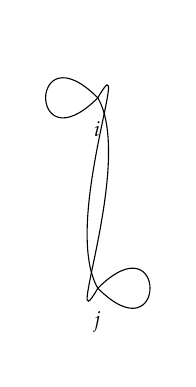
\begin{tikzpicture}[baseline={([yshift=0.2ex]current bounding box.center)}]
      \begin{feynman}
        \vertex (a);
        \vertex (b);
        \diagram {
          a -- [out=135, in=-135, loop, min distance=1.25 cm] a -- 
          [out=60, in=120] b -- [out=45, in=-45, loop, min distance=1.25cm] b 
          -- [out=-120, in=-60] a,
        };
        \vertex [below=0.5em of a] {\(_{i}\)};  
        \vertex [below=0.5em of b] {\(_{j}\)};  
      \end{feynman}
    \end{tikzpicture}
    + \frac{1}{48} 
    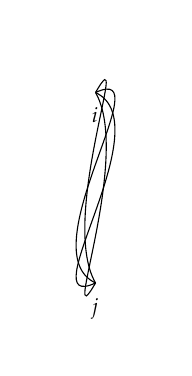
\begin{tikzpicture}[baseline={([yshift=0.2ex]current bounding box.center)}]
      \begin{feynman}
        \vertex (a);
        \vertex (b);
        \diagram {
          a -- 
          [out=60, in=120] b 
          -- [out=-120, in=-60] a,
          a -- [out=25, in=155] b 
          -- [out=-155, in=-25] a,
        };
        \vertex [below=0.2em of a] {\(_{i}\)};  
        \vertex [below=0.2em of b] {\(_{j}\)};  
      \end{feynman}
    \end{tikzpicture}
    \right]\, .
\end{align}
It it clear from the diagrammatic representation that we can
distinguish connected and disconnected contributions. The connected
contributions are represented by connected diagrams, i.e. diagrams
that are made of a single line. The disconnected diagrams are products
of multiple connected parts, and therefore correspond to products of
independent sums over subset of indices. In
Eq.~\ref{eq:PhiFourPartitionFuncOrderLambdaTwo} only the first term in
the bracket in the second line is a disconnected contribution. 

\paragraph{Connected contribution}

Using the Taylor expansion for the logarithm,
\begin{equation}
  \label{eq:TaylorLog}
  \log(1+x) = \sum_{n=1}^\infty (-)^{n+1} \frac{x^n}{n}\, ,
\end{equation}
we can compute
\begin{align}
  \label{eq:PhiFourPartitionFuncConnectOrderLambdaTwo}
  \log\left(Z(\lambda)/Z(0)\right) = 
                    &- \lambda \frac{1}{8} \sum_{i=1}^n \Delta_{ii}^2
                                     +\nonumber \\
                     &+\lambda^2
                    \left[
                    \frac{1}{128} \sum_i \Delta_{ii}^2 \sum_j \Delta_{jj}^2 +
                    \frac{1}{16} \sum_{ij} \Delta_{ii} \Delta_{jj} \Delta_{ij}^2 +
                    \frac{1}{48} \sum_{ij} \Delta_{ij}^4
                    \right] -  \nonumber \\
  &- \lambda^2 \frac{1}{2} \left( - \frac{1}{8}
    \sum_{i=1}^n \Delta_{ii}^2\right)^2 +  O(\lambda^3)\, . 
\end{align}
Eq.~\ref{eq:PhiFourPartitionFuncConnectOrderLambdaTwo} shows
explicitly the cancellation at order $\lambda^2$ between the first
term in the square bracket in the second line, and the last term in
the third line, which comes from squaring the order $\lambda$
contribution when computing the second term in the Taylor expansion in
Eq.~\ref{eq:TaylorLog}. This is a general property, taking the
logarithm of the generating function yields the generating function of
connected conributions. We shall prove this property later in the
course. 

\section{Perturbed Gaussian Correlators}
\label{sec:pert-gauss-corr}

The perturbative treatment discussed above can be extended to compute
moments of the distribution:
\begin{equation}
  \label{eq:lPointCorrPert}
  \langle x_{i_1} \ldots x_{i_\ell}\rangle =
  \frac{1}{Z(\lambda)} 
  \int \dd[n]{x} e^{-S(x;\lambda)} x_{i_1} \ldots x_{i_\ell}\, ,
\end{equation}
which often referred to as an $\ell$-point correlator/function. Let us start
our discussion with a simple example. 

\paragraph{Two-point function}

We need to evaluate
\begin{align}
  \int \dd[n]{x} e^{-S(x;\lambda)} x_{i_1} x_{i_2} &= 
  \int \dd[n]{x} e^{-S_0(x;\lambda)}\, \left[\sum_{k=0}^\infty
  \frac{(-)^k}{k!} \lambda^k V(x)^k \right]\, x_{i_1} x_{i_2} \\
  \label{eq:TwoPointCorrPert}
                                               &=Z(0) \sum_{k=0}^\infty
  \frac{(-)^k}{k!} \lambda^k \langle V(x)^k x_{i_1} x_{i_2}\rangle_0\, ,
\end{align}
where in the second line we have expressed the initial correlator in
terms of correlators computed in the Gaussian theory, denoted as
before by $\langle \ldots \rangle_0$. The Gaussian correlators can be
computed using Wick's theorem as before. We shall consider again a
quartic potential:
\begin{equation}
  V(x) = \frac{1}{4!} \sum_{i=1}^n x_i^4\, ,
\end{equation}
and compute all the terms in Eq.~\ref{eq:TwoPointCorrPert} order by
order in $\lambda$ up to order $\lambda^2$.
\begin{itemize}
\item $O(\lambda^0)$ For $k=0$ we simply get the two-point Gaussian
  correlator: 
  \begin{align}
    \langle x_{i_1} x_{i_2} \rangle_0 = \Delta_{i_1 i_2}\, .
  \end{align}
\item $O(\lambda^1)$ At first order in $\lambda$ we have one insertion
  of $V$:
  \begin{align}
    \langle V(x) x_{i_1} x_{i_2} \rangle_0 = \frac{1}{4!} \sum_{i=1}^n
    \langle x_i^4 x_{i_1} x_{i_2} \rangle_0\, .
  \end{align}
  This Gaussian expectation value involving six factors of $x$ (four
  from the potential, and the two coming from the fact that we compute
  a two-point function) can be evaluated using Wick's
  theorem. There two types of contractions.
  \begin{itemize}
  \item [(i)] $x_1$ is contracted with $x_2$, and the four $x_i$ are
    contracted amongst themselves:
    \begin{align}
      \contraction{}{x_{i_1}}{}{x_{i_2}}
      x_{i_1} x_{i_2} 
      \left(
      \contraction{}{x_{i}}{}{x_{i}}
      \contraction{x_{i} x_{i}}{x_{i}}{}{x_{i}}
      x_{i} x_{i} x_{i} x_{i} +
      \contraction{}{x_{i}}{x_{i}}{x_{i}}
      \contraction[2ex]{x_{i}}{x_{i}}{ x_{i}}{x_{i}}
      x_{i} x_{i} x_{i} x_{i} +
      \contraction{}{x_{i}}{x_{i}x_{i}}{x_{i}}
      \contraction[2ex]{x_{i}}{x_{i}}{}{x_{i}}
      x_{i} x_{i} x_{i} x_{i} 
      \right) = \Delta_{i_1 i_2} \langle x_i^4\rangle_0
      \, ,
    \end{align}
    where we have used the fact that the term inside the bracket on
    the LHS is simply $\langle x_i^4\rangle_0$ --
    cfr. Eq.~\ref{eq:FourPtGaussContract}.
  \item [(ii)] $x_1$ and $x_2$ are contracted with some of the $x_i$;
    there are 12 such contractions:
    \begin{align}
      \contraction{}{x_{i_1}}{x_{i_2}}{x_{i}}
      \contraction[2ex]{x_{i_1}}{x_{i_2}}{x_{i}}{x_{i}}
      x_{i_1} x_{i_2}  x_{i} x_{i} x_{i} x_{i} + \ldots = 
      \Delta_{i i_1} \Delta_{i i_2} \Delta_{i i} \times 4
      \times 3\, .
    \end{align}
  \end{itemize}
  Collecting all terms yields
  \begin{align}
   \frac{1}{4!} \sum_{i=1}^n
    \langle x_i^4 x_{i_1} x_{i_2} \rangle_0 = 
    \Delta_{i_1 i_2} \frac{1}{4!} \sum_{i=1}^n \langle x_i^4\rangle_0
    + \frac{1}{4!} \times 4 \times 3 \sum_{i=1}^n \Delta_{i i_1}
    \Delta_{i i_2} \Delta_{i i} \, .
  \end{align}
\item $O(\lambda^2)$ At this order we need to evaluate
  \begin{align}
    \frac{1}{2!} \langle V(x)^2 x_{i_1} x_{i_2} \rangle_0 = 
    \frac{1}{2!} \frac{1}{(4!)^2} \sum_{i,j=1}^n \langle x_i^4 x_j^4
    x_{i_1} x_{i_2} \rangle_0\, .
  \end{align}
  There are five different types of contractions, each of them coming
  with a given multiplicity. We encourage the interested reader to
  compute those contributions, and check carefully that the correct
  multiplicities are recovered. 
\end{itemize}
Collecting all contributions yields
\begin{align}
  \int \dd[n]{x} e^{-S(x;\lambda)} 
  x_{i_1} x_{i_2} = Z(0) & 
                           \left[
                           \Delta_{i_1 i_2} - \lambda \left(\Delta_{i_1 i_2}
                           \frac{1}{4!} \sum_{i=1}^n \langle
                           x_i^4\rangle_0 +  \frac12 \sum_{i=1}^n
                           \Delta_{i i_1} \Delta_{i i_2} \Delta_{i i} 
                           \right) + \right. \nonumber \\
                         & \left.
                           + \lambda^2 \left( 
                           \frac{1}{2!} \Delta_{i_1 i_2} \frac{1}{(4!)^2}
                           \sum_{i,j=1}^n \langle x_i^4 x_j^4 \rangle_0
                           + \frac{1}{2!} \sum_{i=1}^n \Delta_{i i_1}
                           \Delta_{i i_2} \Delta_{i i}  \frac{1}{4!}
                           \sum_{j=1}^n \langle x_j^4 \rangle_0
                           + \right. \right. \nonumber \\
                         & + \left. \left.
                           \frac{1}{4} \sum_{i,j=1}^n \Delta_{i i_1}
                           \Delta_{i i_2} \Delta_{i j}^2 \Delta_{jj}
                           + \frac{1}{6} \sum_{i,j=1}^n \Delta_{i i_1}
                           \Delta_{j i_2} \Delta_{i j}^3 +
                           \right. \right. \nonumber \\
  \label{eq:TwoPointNotNorm}
                         & + \left. \left.
                           \frac{1}{4} \sum_{i,j=1}^n \Delta_{i i_1}
                           \Delta_{j i_2} \Delta_{i j} \Delta_{ii}\Delta_{jj}
                           \right)
                           \right]\, .
\end{align}
Diagrammatically we have: 
\begin{align}
  \label{eq:TwoPtVacuumIncluded}
  \langle x_{i_1} x_{i_2}\rangle = 
  \frac{Z(0)}{Z(\lambda)} \Bigg[
    \begin{tikzpicture}[baseline={([yshift=1.4ex]current bounding box.center)}]
    \begin{feynman}[inline=(a)]
      \vertex (a);
      \vertex (b);
      \diagram {
        a -- b,
      };
      \vertex [below=0.2em of a] {\(_{i_1}\)};  
      \vertex [below=0.2em of b] {\(_{i_2}\)};  
    \end{feynman}
  \end{tikzpicture}
  + \frac{\lambda}{8}
    \begin{tikzpicture}[baseline={([yshift=-5ex]current bounding box.center)}]
    \begin{feynman}[layered layout, vertical'=i to c]
      \vertex (a);
      \vertex (c); 
      \vertex (b);
      \vertex (i);
      \vertex (j);
      \vertex (k);
      \diagram {
        j -- [draw=none]  i -- [draw=none] k, 
        i -- [out=45, in=-45, loop, min distance=2cm] i --
        [out=135, in=-135, loop, min distance=2 cm] i,
        a -- c -- b, 
        c --[opacity=0.1] i, 
      };
      \vertex [below=0.2em of a] {\(_{i_1}\)};  
      \vertex [below=0.2em of b] {\(_{i_2}\)};  
%      \vertex [below=0.2em of c] {\(c\)};  
      \vertex [below=0.2em of i] {\(_{i}\)};  
    \end{feynman}
  \end{tikzpicture}
  + \frac{\lambda}{2}
    \begin{tikzpicture}[baseline={([yshift=-3ex]current bounding box.center)}]
    \begin{feynman}[layered layout, vertical'=i to c]
      \vertex (a);
      \vertex (b);
      \vertex (i);
      \diagram {
        a -- i -- b, 
        i -- [out=135, in=45, loop, min distance=2cm] i,
      };
      \vertex [below=0.2em of a] {\(_{i_1}\)};  
      \vertex [below=0.2em of b] {\(_{i_2}\)};  
%      \vertex [below=0.2em of c] {\(c\)};  
      \vertex [below=0.2em of i] {\(_{i}\)};  
    \end{feynman}
  \end{tikzpicture}
  + O(\lambda^2)
  \Bigg]\, ,
\end{align}
where for simplicity we have omitted the contribution of order
$\lambda^2$. A diagram that can be factorised as the product of a
subdiagram with external lines and a subdiagram that is made of loops
only is called a {\em vacuum contribution}. For instance the second
diagram inside the bracket in Eq.~\ref{eq:TwoPtVacuumIncluded} is a
vacuum contribution, while the first and third ones are not.

Finally, we need to divide this expression by $Z(\lambda)$ in order to
obtain the two-point correlator as defined in
Eq.~\ref{eq:lPointCorrPert}.  As a result, we obtain a factor of
$Z(0)/Z(\lambda)$ multiplying the expression inside the square bracket
in Eq.~\ref{eq:TwoPointNotNorm}. Inverting
Eq.~\ref{eq:PhiFourPartitionFuncOrderLambdaTwo} for the ratio
$Z(0)/Z(\lambda)$ yields
\begin{align}
 Z(0)/Z(\lambda) &= 
                    1 + \frac{1}{4!} \lambda \sum_{i=1}^n \langle x_i^4\rangle_0 
                    - \frac{1}{2!} \frac{1}{(4!)^2} \lambda^2 \sum_{i,j=1}^n 
                    \langle x_i^4 x_j^4\rangle_0 
                   + \frac{1}{(4!)^2} \lambda^2 \left(\sum_{i=1}^n \langle x_i^4\rangle_0\right)^2
                   + O(\lambda^3) 
\end{align}

\begin{Ex}
  Show that all the vacuum contributions cancel when computing $\langle
  x_{i_1} x_{i_2}\rangle$. The final result is
  \begin{align}
  \int \dd[n]{x} e^{-S(x;\lambda)} 
  x_{i_1} x_{i_2} = Z(0) & 
                           \left[
                           \Delta_{i_1 i_2} - \lambda  \frac12 \sum_{i=1}^n
                           \Delta_{i i_1} \Delta_{i i_2} \Delta_{i i} 
                            + \right. \nonumber \\
                         & \left.
                           + \lambda^2 \left( 
                           \frac{1}{4} \sum_{i,j=1}^n \Delta_{i i_1}
                           \Delta_{i i_2} \Delta_{i j}^2 \Delta_{jj}
                           + \frac{1}{6} \sum_{i,j=1}^n \Delta_{i i_1}
                           \Delta_{j i_2} \Delta_{i j}^3 +
                           \right. \right. \nonumber \\
  \label{eq:TwoPointNorm}
                         & + \left. \left.
                           \frac{1}{4} \sum_{i,j=1}^n \Delta_{i i_1}
                           \Delta_{j i_2} \Delta_{i j} \Delta_{ii}\Delta_{jj}
                           \right)
                           \right]\, .
\end{align}
Write a diagrammatic representation for the contributions $O(\lambda^2)$.
\end{Ex}
This is a general property: when the integral is divided by the
correct normalization factor $1/Z(\lambda)$, all vacuum contributions
cancel.

\section{Generating Functions for the Perturbed Gaussian Measure}
\label{sec:gener-funct-pert}

\paragraph{Correlators}

We can now generalise the idea of a generating function to the case of
a non Gaussian measure. Introducing
\begin{equation}
  \label{eq:GenFunctPert}
  Z(b;\lambda) = \int \dd[n]{x} \exp\left[
    -S(x;\lambda) + (b,x)
    \right]\, ,
\end{equation}
where we introduced the notation
\begin{equation}
  \label{eq:ScalProd}
  (b,x) = \sum_{i=1}^n b_i x_i\, .
\end{equation}
Note that we can also write
\begin{equation}
  \label{eq:GenFunctPertTwo}
  \langle e^{(b,x)} \rangle = Z(b;\lambda)/Z(\lambda)\, .
\end{equation}
The correlators in the perturbed measure are obtained by
differentiation
\begin{equation}
  \label{eq:CorrGenPert}
  \langle x_{i_1} \ldots x_{i_\ell}\rangle = \frac{1}{Z(\lambda)} \left.
  \frac{\partial}{\partial b_{i_1}} \ldots \frac{\partial}{\partial b_{i_\ell}}\,
  Z(b;\lambda)
\right|_{b=0} \, .
\end{equation}

\paragraph{Cumulants}

The logarithm of $Z(b;\lambda)$ is usually denoted $W(b;\lambda)$, 
\begin{equation}
  \label{eq:WGenDef}
  Z(b;\lambda) = e^{W(b;\lambda)}\, ;
\end{equation}
$W(b;\lambda)$ is the generator is the generator of the connected
$\ell$-point correlators, $W_{i_1 \ldots i_\ell}$, i.e. the correlators that can be represented as a single
diagram, with $\ell$ open ends:
\begin{equation}
  \label{eq:DiffWGen}
  W_{i_1 \ldots i_\ell} = \left.
  \frac{\partial}{\partial b_{i_1}} \ldots \frac{\partial}{\partial b_{i_\ell}}\,
  W(b;\lambda)
\right|_{b=0} \, .
\end{equation}
In statistics, the $W_{i_1 \ldots i_\ell}$ are called the {\em
  cumulants} of the probability distribution $e^{-S(x;\lambda)}$.

\end{document}



\chapter{Path Integrals in QM}
\label{chap:lec1}
% !TeX root = ./notes.tex

\documentclass[notes]{subfiles}
   

\begin{document}
\chapter{Path Integrals in QM}
\label{chap:lec1}

\newcommand{\epsstep}{\left(e^{-i \hat{H} \epsilon}\right)}


\section{Preliminaries}
\label{sec:preliminaries-1}

In this lecture we introduce Path Integrals in the context of
QM. Despite the simpler setting (QM compared to QFT), all the
important features of Path Integrals will be discussed. We consider a
point particle in one-dimension, and denote by $\hat{Q}$ the position
operator, and by $\ket{q}$ the eigenstate corresponding to the eigenvalue
$q$:
\begin{equation}
  \label{eq:QEigen}
  \hat{Q} \ket{q} = q \ket{q}\, .
\end{equation}
The completeness condition for the states $\ket{q}$ is
\begin{equation}
  \label{eq:qComplete}
  \int \dd{q}\ketbra{q}{q} = 1\, .
\end{equation}
The aim of this section is to find an expression for the quantum
amplitude $\braket{q't'}{qt}$ for a system in state $\ket{q}$ at time
$t$ to evolve in state $\ket{q'}$ at time $t'$,
\begin{equation}
  \label{eq:AmplitudeDef}
  \braket{q't'}{qt} = \bra{ q'} e^{-i \hat{H} (t'-t)}\ket{q}\, ,
\end{equation}
where $\hat{H}$ is the Hamiltonian of the system. 

\section{Setting Up the Path Integral}
\label{sec:setting-up-path}

In order to proceed with the calculation, let us define $T=t'-t$ to be
the size of the time interval, and $\epsilon=T/n$, where $n$ is an
integer. Then 
\begin{align}
  t_0 &= t \\
  t_k &= t_0 = k \epsilon, \quad \text{for}\ k=1, \ldots, n-1 \\
  t_n &= t + n \epsilon = t'\, .
\end{align}
\begin{align}
  \bra{ q'} e^{-i \hat{H} (t'-t)}\ket{q} &= 
                 \bra{ q'} e^{-i \hat{H} T} \ket{q} \\
               &= \bra{ q'} \left(e^{-i \hat{H} \epsilon}\right)
                 \ldots \left(e^{-i \hat{H} \epsilon}\right) |
                 q\rangle\, ,
\end{align}
where the expression in the second line contains $n$ factors. 

Inserting the completeness relation $n-1$ times,
\begin{align}
  \label{eq:AmplitudeStepOne}
  \braket{q't'}{qt} = \int \prod_{k=1}^{n-1}dq_k\,
  \bra{ q'} \left(e^{-i \hat{H} \epsilon}\right) |q_{n-1}\rangle
  \bra{ q_{n-1}} \left(e^{-i \hat{H} \epsilon}\right) |
  q_{n-2}\rangle \ldots \bra{ q_1} \left(e^{-i \hat{H}
  \epsilon}\right) \ket{q}\, .
\end{align}
For small $\epsilon$ we can expand the exponential to first order and
evaluate the matrix elements:
\begin{align}
  e^{-i \hat{H} \epsilon} &= 1 - i \hat{H} \epsilon + O(\epsilon^2)\\
\hat{H} &= \frac12 \hat{P}^2 + V(\hat{Q})\, ,
\end{align}
From the potential energy we get
\begin{align}
  \bra{ q_k} V(\hat{Q}) | q_{k-1}\rangle &= V(q_{k-1}) \bra{ q_k
                                             } q_{k-1} \rangle \\
                                            &= V\left(\frac{q_k +
                                              q_{k-1}}{2}\right)
                                              \delta(q_k-q_{k-1}) \\
                                            & = \int \frac{dp}{2\pi} V\left(\frac{q_k +
                                              q_{k-1}}{2}\right) 
                                              e^{ip (q_k-q_{k-1})}
\end{align}
In order to evaluate the contribution of the kinetic term, we
introduce eigenstates of the momentum operator $\ket{p}$
\begin{align}
  \hat{P} \ket{p} = p \ket{p} \\
  \braket{q}{p} = e^{ipq}\, ,
\end{align}
and use the completeness of the states $\ket{p}$:
\begin{align}
  \bra{ q_k} \hat{P}^2 | q_{k-1}\rangle = 
  \int \frac{dp}{2\pi}\, p^2 e^{ip(q_k-q_{k-1})}\, .
\end{align}
Hence
\begin{align}
  \bra{ q_k} e^{-i\hat{H}\epsilon} | q_{k-1}\rangle = 
  \int \frac{dp}{2\pi}\, \exp\left\{i\epsilon \left[
  p \frac{q_k-q_{k-1}}{\epsilon} - H\left(p,\tilde{q}\right)
  \right]
  \right\} + O(\epsilon^2)\, ,
\end{align}
where $\tilde{q}=\frac{q_k-q_{k-1}}{2}$. Therefore
\begin{align}
  \braket{q't'}{qt} =& \lim_{n\to\infty} \int \prod_{k=1}^{n-1}dq_k\, 
  \prod_{j=1}^{n} \frac{dp_j}{2\pi}\, \times \\
  &\times \exp \left\{
    i\epsilon \sum_{m=1}^{n} \left[
    p_m \frac{q_m-q_{m-1}}{\epsilon} - H\left(p_m, 
    \frac{q_m+q_{m-1}}{2}\right)
    \right]
    \right\}\, ,
\end{align}
where $q_0 = q$, and $q_n = q'$. The limit above defines the {\em
  path integral} evaluation of the quantum amplitude, which we denote 
\begin{align}
  \label{eq:PathIntDefZero}
  \braket{q't'}{qt} = 
  \int \mathcal{D}q \mathcal{D}p \exp \left\{
  i \int_t^{t'} \dd{\tau} \left[
  p \dot{q} - H(p,q)
  \right]
  \right\}\, .
\end{align}

\section{Quadratic P dependence}
\label{sec:quadr-kinet-term}

For hamiltonians like the one above, \ie hamiltonians that are only
quadratic in the momentum $\hat{P}$, the expression above can be
simplified by performing the integral over the momenta $p_j$:
\begin{align}
  \int \frac{dp}{2\pi}\, \exp\left\{
  i\epsilon\left[
  p \left(\frac{q_k-q_{k-1}}{\epsilon}\right) - \frac12 p^2
  \right]
  \right\} = \left(2\pi i \epsilon\right)^{-\nicefrac{1}{2}}\,
  \exp\left\{i\epsilon
  \frac12\left(\frac{q_k-q_{k-1}}{\epsilon}\right)^2\right\}\, .
\end{align}
Using this result, we can rewrite the path integral in
\Eqref{eq:PathIntDefZero} as
\begin{align}
  \label{eq:PathIntDefOne}
  \braket{q't'}{qt} = \lim_{n\to\infty}
  \left(2\pi i \epsilon\right)^{-\nicefrac{n}{2}}\,
  \int \prod_{k=1}^{n-1}dq_k\, 
  \exp \left\{
  i \epsilon \sum_{m=1}^{n}
  \, \left[
  \frac12 \left(\frac{q_m-q_{m-1}}{\epsilon}\right)^2
  -V\left(\frac{q_m+q_{m-1}}{2}\right)
  \right]
  \right\}\, .
\end{align}
Assuming that the limit exists, we have obtained the definition of the
path integral as an integral over the position of the system only: 
\begin{align}
  \label{eq:PathIntDef}
  \braket{q't'}{qt} = 
  \int_{q,q'} \mathcal{D}q \exp \left\{
  i \int_t^{t'} \dd{\tau}  \mathcal{L}(q,\dot{q})
  \right\}\, ,
\end{align}
where $\mathcal{L}$ is the lagrangian of the system. Note that the
suffix of the integral keeps track of the initial- and final-state
configurations $q$ and $q'$. 

\section{Correlators}
\label{sec:correlators}

We are now going to work out expressions for the matrix element of the
position operator inbetween the initial and final state considered
above. 

\subsection{One-point Function}
\label{sec:one-point-function}

The first example that we are going to consider is the matrix element
\begin{align}
  \label{eq:OnePtDef}
  \bra{ q't'} \hat{Q}(\bar{t}) | q t\rangle = 
  \bra{ q'} e^{-i \hat{H}(t'-t)} \hat{Q} e^{-i \hat{H}(\bar{t}-t)}
  \ket{q}\, ,
\end{align}
where we assume $t<\bar{t}<t'$, and we have used
\begin{equation}
  \label{eq:HeisenOpEvol}
  \hat{Q}(t) = e^{i\hat{H} t} \hat{Q} e^{-i\hat{H} t}\, .
\end{equation}
Proceeding as we did in the previous section, we can write
\begin{align}
  \label{eq:CorrOne}
  \bra{ q't'} \hat{Q}(\bar{t}) | q t\rangle = 
  \bra{q'} \epsstep \ldots \epsstep \hat{Q} \epsstep \ldots
  \epsstep \ket{q}\, ,
\end{align}
where we assumed that $\bar{t}=t_k$, and the first and second ellipses
denote respectively $(n-k)$, and $k$ factors of $\epsstep$. Performing
the same manipulations as before we obtain
\begin{align}
  \bra{ q't'} \hat{Q}(\bar{t}) | q t\rangle =& 
  \lim_{n\to\infty} \int \prod_{k=1}^{n-1}dq_k\, 
  \prod_{j=1}^{n} \frac{dp_j}{2\pi}\, q_k \times \\
  &\times \exp \left\{
    i\epsilon \sum_{m=1}^{n} \left[
    p_m \frac{q_m-q_{m-1}}{\epsilon} - H\left(p_m, 
    \frac{q_m+q_{m-1}}{2}\right)
    \right]
    \right\}\, .
\end{align}
Note that now there is an extra factor of $q_k$ in the integrand,
corresponding to the insertion of the operator $\hat{Q}(\bar{t})$. The
limit above  is denoted
\begin{align}
  \bra{ q't'} \hat{Q}(\bar{t}) | q t\rangle &= 
  \int \mathcal{D}q \mathcal{D}p \, q(\bar{t}) 
  \exp \left\{
  i \int_t^{t'} \dd{\tau} \left[
  p \dot{q} - H(p,q)
  \right]
  \right\}\\
&= \int_{qq'} \mathcal{D}q \, q(\bar{t}) 
  \exp \left\{
  i \int_t^{t'} \dd{\tau} \mathcal{L}(q,\dot{q})
  \right\}\, .
\end{align}

\subsection{Two-point function}
\label{sec:two-point-function}

Let us now consider the slightly more complicated case of the matrix
element of the product of two position operators
\begin{align}
  \label{eq:TwoPtDef}
  \bra{q't'} \hat{Q}(\bar{t}_1) \hat{Q}(\bar{t}_2)\ket{qt}\, , 
\end{align}
where now we assume $\bar{t}_1=t_k$, $\bar{t}_2=t_\ell$,
$t<\bar{t}_2<\bar{t}_1<t'$. We can write this correlator as:
\begin{align}
    \bra{q't'} \hat{Q}(\bar{t}_1) \hat{Q}(\bar{t}_2)\ket{qt} = 
  \bra{q'} \epsstep \dots \hat{Q} \ldots \hat{Q} \ldots \epsstep
  \ket{q}\, ,
\end{align}
where the three ellipses here denote respectively $(n-k)$, $(k-\ell)$,
and $\ell$ factors of $\epsstep$. Proceeding exactly as above yields: 
\begin{align}
  \label{eq:TwoPtPathInt}
  \bra{q't'} \hat{Q}(\bar{t}_1) \hat{Q}(\bar{t}_2)\ket{qt} = 
  \int_{qq'} \mathcal{D}q\, q(\bar{t}_1) q(\bar{t}_2) 
  \exp \left\{
  i \int_t^{t'} \dd{\tau} \mathcal{L}(q,\dot{q})
  \right\}\, .
\end{align}

There is a subtlety here that it is worth noting. The ordering of
times in \Eqref{eq:TwoPtDef} matters, while it clearly does not in the
RHS of \Eqref{eq:TwoPtPathInt} where $q(\bar{t}_1)$ and $q(\bar{t}_1)$
are just integration variables. If $\bar{t}_2>\bar{t}_1$, then the RHS
of \Eqref{eq:TwoPtPathInt} corresponds to
\begin{align}
  \bra{q't'} \hat{Q}(\bar{t}_2) \hat{Q}(\bar{t}_1) \ket{qt}\, .
\end{align}
Both results can be summarised as
\begin{align}
  \label{eq:TOrderPathInt}
  \bra{q't'} T\left(\hat{Q}(\bar{t}_1) \hat{Q}(\bar{t}_2)
  \right)\ket{qt} = 
  \int_{qq'} \mathcal{D}q\, q(\bar{t}_1) q(\bar{t}_2) 
  \exp \left\{
  i \int_t^{t'} \dd{\tau} \mathcal{L}(q,\dot{q})
  \right\}\, ,
\end{align}
where we have introduced the T-ordered product of operators: 
\begin{align}
  \label{eq:TOrderDef}
   T\left(\hat{Q}(t) \hat{Q}(t')\right) = \theta(t-t') \hat{Q}(t)
  \hat{Q}(t') + \theta(t'-t) \hat{Q}(t') \hat{Q}(t)\, .
\end{align}

You can easily verify that the derivation can be extended to
an arbitrary number of insertions of the operator $\hat{Q}$:
\begin{align}
\label{eq:TOrderNPt}
\bra{q't'} T\left(\hat{Q}(\bar{t}_1) \ldots \hat{Q}(\bar{t}_n)
  \right)\ket{qt} = 
  \int_{qq'} \mathcal{D}q\, q(\bar{t}_1) \ldots q(\bar{t}_n) 
  \exp \left\{
  i \int_t^{t'} \dd{\tau} \mathcal{L}(q,\dot{q})
  \right\}\, .
\end{align}

\section{Generating functional}
\label{sec:gener-funct}

\subsection{Functional derivative}
\label{sec:funct-deriv}

Consider a functional $F$ that associates a number, which we denote
$F[u]$, to a given function $u(x)$. The functional derivative
describes the change of the functional to an infinitesimal variation
of the function $u$: 
\[
  u(x) \mapsto u(x) + \delta u(x)\, .
\]
We define
\begin{equation}
  \label{eq:FuncDer}
  \delta F = F[u+\delta u] - F[u] = \int dx\, \frac{\delta F}{\delta
    u(x)} \delta u(x)\, .
\end{equation}
You can see the analogy to the case of a function of several
variables, where the variation to a change $\delta x_k$ in the
variables is given by
\begin{equation}
  \label{eq:NormDer}
  \delta F = F(x+\delta x) - F(x) = \sum_k \frac{\partial F}{\partial
    x_k} \delta x_k\, .
\end{equation}
In particular we have
\begin{equation}
  \label{eq:DiracDelta}
  \frac{\delta}{\delta f(x)} f(y) = \delta(x-y)\, , 
\end{equation}
again to be compared with its discrete analogue
\begin{equation}
  \label{eq:KroneckerDelta}
  \frac{\partial}{\partial x_j} x_i = \delta_{ij}\, .
\end{equation}

\subsection{Sources in the path integral}
\label{sec:sourc-path-integr}

Let $f(t)$ and $h(t)$ be two functions, we can add so-called source
terms to the path integral, and define
\begin{equation}
  \label{eq:PathIntegralSources}
  \braket{q't'}{qt}_{f,h} = \int \mathcal{D}p \mathcal{D}q\,\exp 
  \left\{
    i \int_{t}^{t'} d\tau \left[
      p(\tau) \dot{q}(\tau) - H(p(\tau),q(\tau)) + f(\tau) q(\tau) +
      h(\tau) p(\tau)
      \right]
  \right\}\, .
\end{equation}
Taking functional derivatives with respect to the source fields yields
e.g.
\begin{align}
  \left(\frac{1}{i} \frac{\delta}{\delta f(\bar\tau)} \right)&
  \braket{q't'}{qt}_{f,h} = \nonumber \\
  =&\int \mathcal{D}p \mathcal{D}q\,
  q(\bar{\tau})\,
  \exp \left\{
  i \int_{t}^{t'} d\tau \left[
  p(\tau) \dot{q}(\tau) - H(p(\tau),q(\tau)) + f(\tau) q(\tau) +
  h(\tau) p(\tau)
  \right]
  \right\}\, ,
\end{align}
\begin{align}
  \left(\frac{1}{i} \frac{\delta}{\delta f(\bar\tau_1)} \right)&
  \left(\frac{1}{i} \frac{\delta}{\delta f(\bar\tau_2)} \right)
  \braket{q't'}{qt}_{f,h} = \nonumber \\
  =&\int \mathcal{D}p \mathcal{D}q\,
  q(\bar{\tau}_1) q(\bar{\tau}_2)\,
  \exp \left\{
  i \int_{t}^{t'} d\tau \left[
  p(\tau) \dot{q}(\tau) - H(p(\tau),q(\tau)) + f(\tau) q(\tau) +
  h(\tau) p(\tau)
  \right]
  \right\}\, , 
\end{align}
and similarly for the derivatives with respect to $h$ pulling down
factors of $p$ in the integrand. 

As we have seen in the previous section, we have
\begin{align}
  \bra{q't'}  T\left(
  \hat{Q}(t_1)\ldots \hat{Q}(t_n) 
  \right)
  \ket{qt} =& \nonumber \\
  =& \left(\frac{1}{i} \frac{\delta}{\delta f(t_1)} \right) \ldots
    \left(\frac{1}{i} \frac{\delta}{\delta f(t_n)} \right)\,
    \braket{q't'}{qt}_{f,h}\Bigg|_{f=h=0}\, .
\end{align}

\section{Projection onto the ground state}
\label{sec:proj-onto-ground}

It is useful to be able to compute the amplitude for the system to
evolve from the vacuum state at time $t$ into the vacuum state at time
$t'$ under the action of the external sources $f,h$. Having computed
$\braket{q't'}{qt}$, the above amplitude is given by
\begin{align}
  \label{eq:VacToVacAmpl}
  \braket{0,t'}{0,t} = 
  \int dq dq'\, \phi_0(q')^*\, \braket{q't'}{qt}_{f,h}\, \phi_0(q)\, ,
\end{align}
where $\phi_0(q)=\braket{q}{0}$ is the wave function of the ground
state, and $\ket{n}$ denote the eigenstates of the
Hamiltonian. \Eqref{eq:VacToVacAmpl} yields the right amplitude, but
requires the convolution of $\braket{q't'}{qt}$ with the ground state
wave function. We shall now describe a procedure that allows the
compute the vacuum-to-vacuum amplitude directly as a path integral. 

The energy eigenstates are
\begin{equation}
  \label{eq:EnEigen}
  \hat{H} \ket{n} = E_n \ket{n}\, ,
\end{equation}
and their wave functions are denoted as
\begin{equation}
  \label{eq:EnEigenFun}
  \phi_n(q) = \braket{q}{n}\, .
\end{equation}
We assume that the vacuum energy vanishes, $E_0=0$. We want to
evaluate the amplitude
\begin{equation}
  \label{eq:LargeQAmpl}
  \braket{Q'T'}{QT}_{f,h}
\end{equation}
where the sources $h$ and $f$ have support in the interval $[t,t']$,
with $T < t < t' < T'$. The sources behind switched off between $T$
and $t$, we can readily compute
\begin{align}
  \braket{qt}{QT} &= \int \mathcal{D}q \mathcal{D}p \,
                    \exp\left\{
                    i \int_T^t \dd{\tau} \left[
                    p \dot{q} - H(p,q)
                    \right]
                    \right\} \\
  &= \bra{q} \exp\left[-i \hat{H} (t-T)\right] \ket{Q} \\
  &= \sum_n \phi_n(q) \phi_n(Q)^* e^{-i E_n(t-T)}\, .
\end{align}
We can now analytically continue the result to $T_I=(1-i\epsilon)T$,
and consider the limit $T\to -\infty$:
\begin{align}
  \lim_{T\to -\infty} \braket{qt}{QT_I} = \phi_0(q) \phi_0(Q)^*\, .
\end{align}
A similar result can be obtained for $\braket{Q'T'}{q't'}$. We can
therefore write
\begin{align}
  \braket{Q'T'}{QT}_{f,h} = \int \dd{q'} \dd{q} \braket{Q'T'}{q't'} \braket{q't'}{qt}_{f,h}
  \braket{qt}{QT}\, .
\end{align}
And therefore
\begin{align}
 \lim_{\substack{T'\to\infty\\T\to -\infty}} 
\frac{\braket{Q', (1-i\epsilon)T'}{Q, (1-i\epsilon)T}_{f,h}}{\phi_0(Q)^* \phi_0(Q')} = 
  \int \dd{q'}\dd{q} \phi_0(q')^* \braket{q't'}{qt}_{f,h} \phi_0(q)\, .
\end{align}
The expresson on the RHS is the vacuum-to-vacuum amplitude,
$\braket{0,t'}{0,t}_{f,h}$, that we want to compute. The expression on
the LHS is the limit of the path integral for $T\to\infty$,
$T'\to\infty$. The only dependence on the boundary values $Q$ and $Q'$
appears in the denominator on LHS: it is a normalization factor
independent of $f$ and $h$, which disappears when taking derivatives
with respect to the sources. Instead of analytically continuing to
complex values of $T$ and $T'$, we can simply add an imaginary part to
the Hamiltonian,
\begin{equation}
  \label{eq:ComplexTermHam}
  \hat{H} \to (1-i\epsilon) \hat{H}\, .
\end{equation}
Taking the limit $T\to\infty$, $T'\to\infty$, we obtain the amplitude
\begin{equation}
  \label{eq:VacToVac}
  \braket{0}{0}_{f,h} = \int \mathcal{D}p \mathcal{D}q \, \exp
  \left\{
    i \int_{-\infty}^\infty \dd{\tau} \Big[
      p \dot{q} - (1-i\epsilon) H(p,q) + f q + h p 
      \Big]
  \right\}
\end{equation}


\section{Weyl ordering}
\label{sec:weyl-ordering}

If we are interested in more general Hamiltonians, with terms that
involve products of $\hat{P}$ and $\hat{Q}$, then we need to give a
prescription for the ordering of the operators in the Hamiltonian, so
that the quantum mechanical amplitude is actually described by the
path integral. 

As discussed by Berezin in 1971, the mid-point prescription we adopted
in \Eqref{eq:PathIntDefOne} is equivalent to the Weyl-ordering of the
Hamiltonian. 

The Weyl product of two operators $\hat{A}$ and $\hat{B}$ is defined
by considering the operator $\left(\alpha \hat{A} + \beta
  \hat{B}\right)^n$, and expanding it in powers of $\alpha$ and $\beta$: 
\begin{equation}
  \label{eq:WeylOrder}
  \left(\alpha \hat{A} + \beta
    \hat{B}\right)^n = \sum_k \frac{n!}{k! l!}\, 
  \alpha^k \beta^l\, \left[\hat{A}^k
    \hat{B}^l\right]\, .
\end{equation}
The quantity in the square bracket is the Weyl ordered product of
$\hat{A}^k$ and $\hat{B}^l$. 
\end{document}


\chapter{Path Integrals for Scalar Fields}
\label{cha:path-integr-scal}
% !TeX root = ./notes.tex

\documentclass[notes]{subfiles}


\begin{document}
  \chapter{Path Integrals for Scalar Fields}
  \label{cha:path-integr-scal}
  \section{Free field theory}
  \label{sec:real-scalar-field}

  The lagrangian for a free real scalar field $\phi$ is given by
  \begin{equation}
    \label{eq:RealScalLagr}
    \mathcal{L}_0\left(\phi(x)\right)=
    \frac12 \partial_\mu \phi(x) \partial^\mu \phi(x) - 
    \frac12 m^2 \phi(x)^2\, .
  \end{equation}
  The Euler-Lagrange equations of motion, 
  \begin{equation}
    \label{eq:EulerLagrange}
    \partial_\mu \frac{\partial \mathcal{L}_0}{\partial\left(\partial_\mu \phi(x)\right)} 
    - \frac{\partial \mathcal{L}_0}{\partial \phi(x)}\, ,
  \end{equation}
  yields the Klein-Gordon equation
  \begin{equation}
    \label{eq:KleinGordonScal}
    \partial_\mu \partial^\mu \phi(x) + m^2 \phi(x) = \left( \partial^2 + m^2 \right) \phi(x) = 0\, . 
  \end{equation}

  \paragraph{Lorentz Invariance}

  Note that $\mathcal{L}_0$ is invariant under Lorentz transformations:
  \begin{equation}
    \label{eq:LorentzTransfScal}
    x^\mu \mapsto x'^\mu =  \Lambda^\mu_\nu x^\nu\, , \quad \quad 
    \phi(x) \mapsto \phi'(x) = \phi(\lambda^{-1}x)\, .
  \end{equation}

  \paragraph{Conjugate Momentum} 

  The momentum conjugate to $\phi(x)$ can be readily computed:
  \begin{align}
    \label{eq:ScalMom}
    \Pi(x) &= \frac{\partial \mathcal{L}_0}{\partial (\partial_0\phi(x))} \\
    &= \partial_0 \phi(x) = \dot{\phi}(x)\, .
  \end{align}
  And therefore the Hamiltonian is 
  \begin{align}
    \mathcal{H} &= \Pi(x) \dot{\phi}(x) - \mathcal{L}_0\left(\phi(x)\right) \\
    &= \frac12 \Pi(x)^2 + \frac12 \sum_{k=1}^3 \left(\partial_k \phi(x)\right)^2
      + \frac12 m^2 \phi(x)^2\, .
  \end{align}
  The quadratic Hamiltonian is the generalization of the harmonic oscillator to the case where we have an infinite number of canonical coordinates, indexed by the continuous spatial coordinate $\bfx$. 

  \section{Path Integral }
  \label{sec:path-integral}

  The vacuum-to-vacuum amplitude in the presence of a source field $J(x)$ is the straightforward generalization of the expression we have derived for the quantum mechanical system. The correspondence between the two systems is as follows:

  

  \begin{center}
    \begin{tabular}[!h]{lcl}
      $q(t)$ & $\longrightarrow$ & $\phi(t,\bfx)$ \\
      $\hat{Q}(t)$ & $\longrightarrow$ & $\hat{\phi}(t,\bfx)$ (operator) \\
      $f(t)$ & $\longrightarrow$ & $J(t,\bfx)$ (source) \\
    \end{tabular}
  \end{center}

  

  The projection onto the ground state is implemented by the $\epsilon$
  trick that we introduced in the case of quantum mechanics, \ie by
  replacing the Hamiltonian with $(1-i\epsilon) H$. In the case of the
  scalar field theory, this is conveniently achieved by the substitution
  $m^2 \mapsto m^2 - i\epsilon$. In all subsequent formulae we will
  assume that the squared mass has an infinitesimal (negative) imaginary
  part.   

  By analogy with the QM computation, we can write the expression for
  the path integral representation of the vacuum amplitude 
  \begin{align}
    \label{eq:ScalPathIntDef}
    Z_0[J] = \braket{0}{0}_J = 
    \int \mathcal{D}\phi\, \exp\bigg\{
    i \Big[
    S_0[\phi] + J\cdot \phi
    \Big]
    \bigg\}\, ,
  \end{align}
  where 
  \begin{align}
    S_0[\phi] = \int d^Dx\, \mathcal{L}_0\left(\phi(x)\right)\, ,
    \quad
    J \cdot \phi = \int d^Dx\, J(x) \phi(x)\, .
  \end{align}
  For a free theory the integral in \Eqref{eq:ScalPathIntDef} is a
  Gaussian integral, similar to the ones we have seen in the first
  lecture. In order to make the correspondence more explicit, we can
  write the action as
  \begin{align}
    S_0[\phi] = \int d^Dx d^Dx'\, \phi(x) K(x,x') \phi(x') + 
    \int d^Dx\, J(x) \phi(x)\, ,
  \end{align}
  where we recognise a quadratic term, with $K(x,x')$ playing the role
  of $A_{ij}$, and $J(x)$ playing the role of the lienar term $b_i$. The
  explicit expression for the kernel $K$ is
  \begin{align}
    K(x,x') = \Big[ -\partial^2 - m^2\Big] \delta(x-x')\, .
  \end{align}

  It is convenient to work in momentum space, where the kernel
  in the action is diagonal. Introducing the Fourier transforms
  \begin{equation}
    \label{eq:ScalFieldFourier}
    \phi(x) = \int \frac{d^Dp}{(2\pi)^D}\, e^{-i p\cdot x}\,
    \tilde{\phi}(p)\, ,
  \end{equation}
  we can rewrite the kinetic term: 
  \begin{align}
    \int d^Dx\, \partial_\mu \phi(x) \partial^\mu \phi(x) 
    &= \int d^Dx\, \int_{p,p'}\, (-ip_\mu) e^{-ip \cdot x} \tilde{\phi}(p) 
    (-ip'^\mu) e^{-ip'\cdot x} \tilde{\phi}(p') \\
    &= \int_p \, p^2 \tilde{\phi}(p) \tilde{\phi}(-p)
      =  \int_p p^2 \left|\tilde{\phi}(p)\right|^2\, ,
  \end{align}
  where we have introduced the notation
  \begin{align}
    \int_p  = \int \frac{d^Dp}{(2\pi)^D}\, ,
  \end{align}
  and used the fact that $\phi(x)$ is real, and hence $\tilde{\phi}(-p) =
  \tilde{\phi}(p)^*$. Hence the action for the free field in momentum
  space can be written as
  \begin{align}
    \label{eq:ScalFreeMomSpace}
    S_0[\phi] = \frac12 \int_p \bigg\{
    \tphi(-p) \left[p^2 - m^2 + i \epsilon\right] \tphi(p) +
    \tj(p) \tphi(-p) + \tj(-p) \tphi(p)
    \bigg\}\, .
  \end{align}
  Note that the contribution from the $\epsilon$ term to the exponential
  is 
  \begin{align}
    \exp\bigg\{
    -\epsilon \int_p \left|\tphi(p)\right|^2
    \bigg\}\, ,
  \end{align}
  which clearly is convergent for large values of $|\tphi(p)|$.
  It is also important to note that the action for the free field is
  quadratic, and the kernel is diagonal in momentum space. Therefore the
  path integral for the free field is a simple extension of the Gaussian
  integrals that we have been discussing in previous lectures. We will
  use these previous results extensively. 

  The Gaussian integral can be computed by performing the \emph{usual}
  shift of the integration variables
  \[
    \tilde{\chi}(p) = \tphi(p) + \frac{\tj(p)}{p^2-m^2+i\epsilon}\, ,
  \]
  so that
  \begin{align}
    S_0[\chi] = 
    \frac12 \int_p \bigg\{
    \tchi(-p) \left[p^2-m^2+i\epsilon\right] \tchi(p)
    + \tj(-p) \frac{1}{p^2-m^2+i\epsilon} \tj(p)
    \bigg\} \,.
  \end{align}
  Up to a normalization factor
  \begin{align}
    Z_0[J] &\propto \exp \frac{i}{2} \int_p \tj(-p)
            \frac{1}{p^2-m^2+i\epsilon} \tj(p) \\
    &= \exp \frac{i}{2} \int d^Dx d^Dx'\,  J(x) \Delta(x,x') J(x') \, ,
  \end{align}
  where
  \begin{align}
    \Delta(x,x') = \Delta(x-x') = 
    \int_p e^{-i p\cdot (x-x')} \frac{1}{p^2-m^2+i\epsilon}\, .
  \end{align}
  You can easily verify that $\Delta=K^{-1}$, \ie
  \begin{align}
    \int d^Dz \, K(x,z) \Delta(z,x') = \delta(x-x')\, .
  \end{align}
  $\Delta$ is called the \emph{Feynman propagator}.

  Following our previous derivations for Gaussian integrals and QM, you
  can show that
  \begin{align}
    \bra{0} T \phi(x_1) \phi(x_2) \ket{0}_0 &= 
    \left(\frac{1}{i} \frac{\delta}{\delta J(x_1)}\right)
    \left(\frac{1}{i} \frac{\delta}{\delta J(x_2)}\right)
    Z_0[J]\Big|_{J=0} \\ 
    &= \frac{1}{i} \Delta(x_1-x_2)\, .
  \end{align}
  Further correlators are obtained by taking further more derivatives
  \begin{align}
    \bra{0} T \phi(x_1) \ldots \phi(x_n) \ket{0}_0 
    &= 
      \left(\frac{1}{i} \frac{\delta}{\delta J(x_1)}\right)
      \ldots
      \left(\frac{1}{i} \frac{\delta}{\delta J(x_n)}\right)
      Z_0[J]\Big|_{J=0} \, .
  \end{align}
  They can be computed in the free theory using Wick's theorem, again
  following the arguments we used for Gaussian integrals: 
  \begin{align}
    \bra{0} T \phi(x_1) \phi(x_2) \phi(x_3) 
    &\phi(x_4) \ket{0}_0 
      = \frac{1}{i^2} \left[
      \Delta(x_1-x_2) \Delta(x_3-x_4) + \right. \nonumber \\
    & \left. + \Delta(x_1-x_2) \Delta(x_3-x_4) + 
      \Delta(x_1-x_2) \Delta(x_3-x_4)
      \right]\, .
  \end{align}

  \section{Interacting theory}
  \label{sec:interacting-theory}

  Let us now add an interaction term in the lagrangian:
  \begin{align}
    \mathcal{L}\left(\phi(x)\right) = 
    \mathcal{L}_0\left(\phi(x)\right) + V\left(\phi(x)\right)\, .
  \end{align}
  We are going to consider several examples, \eg
  \begin{align}
    V\left(\phi(x)\right) = \frac{1}{3!} g \phi(x)^3\, .
  \end{align}
  What is the dimension of the coupling $g$ as a function of $D$?

  Denoting by $S_0[\phi]$ the action of the free theory, we can write
  the path integral for the interacting theory
  \begin{align}
    Z[J] = \braket{0}{0}_J = \int \mathcal{D}\phi\, 
    \exp\Bigg\{i \left( S_0[\phi] + \int d^Dx\,  V\left(\phi(x)\right) 
    + J \cdot \phi \right) \Bigg\}\, .
  \end{align}
  By performing the same manipulations that we discusssed for 
  gaussian integrals we obtain
  \begin{align}
    Z[J] &= \exp \Bigg\{i \int d^Dx\,  
          V\left(\frac{1}{i}\frac{\delta}{\delta J(x)}\right) \Bigg\}\, 
          \int \mathcal{D}\phi\, 
          \exp\Bigg\{i \left( S_0[\phi]  
          + J \cdot \phi \right) \Bigg\} \\
        &= \exp \Bigg\{i \int d^Dx\,  
          V\left(\frac{1}{i}\frac{\delta}{\delta J(x)}\right) \Bigg\}\, 
          Z_0[J]\, .
  \end{align}
  A useful expression is obtained by expanding both exponentials
  \begin{align}
    Z[J] \propto 
    \sum_{V=0}^\infty & \frac{1}{V!} \left[
                        \frac{i g}{3!} \int d^Dx\, 
                        \left(\frac{1}{i}\frac{\delta}{\delta J(x)}\right)^3
                        \right]^V \times \\
    \label{eq:DoubleExpExp}
                      & \sum_{P=0}^\infty \frac{1}{P!} \left[
                        \frac{i}{2} \int d^Dy\, d^Dz\, 
                        J(y) \Delta(y-z) J(z)
                        \right]^P
  \end{align}
  Consider now the contribution for fixed values of $P$ and $V$, we are
  left with $E=2P-3V$ sources. Let us look at the details that enter in
  this contribution. 
  \begin{itemize}
  \item the overall factor of '$i$': 
    \begin{align}
      i^V \left(\frac{1}{i}\right)^{3V} i^P = i^{P-2V} = i^{E-P+V}\, .
    \end{align}
  \item derivatives acting on sources: 
    \begin{align}
      \frac{(2P)!}{E!}\ \mathrm{combinations}\, .
    \end{align}
  \end{itemize}
  Many contractions yield the same result, which we will represent again
  using a diagrammatic representation. 
  \begin{itemize}
  \item Propagators, $\Delta(x-y)$, are
    represented by a line connecting the points $x$ and $y$. 
    \begin{equation}
      \label{eq:DeltaXYFeynDiag}
      \frac{1}{i}\Delta(x-y) = 
      \begin{tikzpicture}[baseline={([yshift=1.4ex]current bounding box.center)}]
        \begin{feynman}[inline=(a)]
          \vertex (a);
          \vertex (b);
          \diagram {
            a -- b,
          };
          \vertex [below=0.2em of a] {\(_{x}\)};  
          \vertex [below=0.2em of b] {\(_{y}\)};  
        \end{feynman}
      \end{tikzpicture}\, .
    \end{equation}
    External sources are represented with a solid dot at the end of a
    line. Note that the solid dot includes the integration over $x$. 
    \begin{equation}
      \label{eq:CurrentXFeynDiag}
      i \int d^Dx\, J(x) = 
      \begin{tikzpicture}[baseline={([yshift=0.2ex]current bounding box.center)}]
        \begin{feynman}[inline=(a)]
          \vertex (a);
          \vertex (b);
          \diagram {
            a [dot] -- b,
          };
          \vertex [below=0.7em of a] {\(_{x}\)};  
          % \vertex [below=0.2em of b] {\(y\)};  
        \end{feynman}
      \end{tikzpicture}\, .
    \end{equation}
  \item Interactions are represented as three-prong vertices, again
    including the integration over x.
    \begin{equation}
      \label{eq:VertXFeynDiag}
      i g \int d^Dx\,  = 
      \begin{tikzpicture}[baseline={([yshift=0.2ex]current bounding box.center)}]
        \begin{feynman}[small, inline=(v)]
          \vertex (v);
          \vertex [above=of v](i1);
          \vertex [below right=of v](i2); 
          \vertex [below left=of v](i3); 
          \diagram {
            (i1) -- (v),
            (v) -- (i2),
            (v) -- (i3),
          };
        \end{feynman}
      \end{tikzpicture}\, .
    \end{equation}  
  \end{itemize}
  We can then count the number of contractions that yield a particular
  diagram, \ie. a particular contribution. Assuming that there is no
  symmetry in the structure of the diagram, we have the following
  possibilities. 
  \begin{itemize}
  \item permutations of the functional derivatives: $(3!)^V$;
  \item permutations of the vertices: $V!$;
  \item permutations of the sources at the end of propagators: $2^P$;
  \item permutations of propagators: $P!$.
  \end{itemize}
  These factors match \emph{exactly} the ones that appear in the
  expansions of the exponentials above. So in the absence of any
  symmetry in the diagram, each diagram contributes to
  Eq.~(\ref{eq:DoubleExpExp}) multiplied by a factor of 1. However, this
  procedure results in a double counting of the possible contributions
  if there are symmetries in the structure of the diagram, \ie if a
  permutation of derivatives results in the same operations as a
  permutation of the sources. 

  

  \noindent
  \textbf{Example:} let us consider the case $P=2$, $V=1$, and hence
  $E=4-3=1$. The term in the double expansion is
  \begin{align}
    \frac{i g}{3!} \int d^Dx\, 
    & \left(\frac{1}{i}\frac{\delta}{\delta J(x)}\right)
      \left(\frac{1}{i}\frac{\delta}{\delta J(x)}\right)
      \left(\frac{1}{i}\frac{\delta}{\delta J(x)}\right)\,
      \frac{1}{2!} \frac{i}{2}\, 
      \int d^Dy_1\, d^Dz_1\, J(y_1) \Delta(y_1-z_1) J(z_1) \nonumber \\  
    & \times \int d^Dy_2\, d^Dz_2\, J(y_2) \Delta(y_2-z_2) J(z_2)\, .
  \end{align}
  It can be rewritten as 
  \begin{align}
    g \frac{1}{3! \times 2! \times 2 \times 2}\, 
    & \int d^Dx\, d^Dy_1\, d^Dz_1\, d^Dy_2\, d^Dz_2\, 
      \Delta(y_1-z_1) \Delta(y_2-z_2) \times \nonumber \\
    & \times \left(\frac{\delta}{\delta J(x)}\right)
      \left(\frac{\delta}{\delta J(x)}\right)
      \left(\frac{\delta}{\delta J(x)}\right)\,
      J(y_1) J(z_1) J(y_2) J(z_2)\, .
  \end{align}
  We are going to count the possible contractions in two different ways. 
  \begin{enumerate}
  \item Just counting: there are 4 possible choice to decide which $J$
    is not paired with a derivative. Then there are $3!$ possible ways
    of pairing the derivatives with the three $J$s. The derivatives
    acting on the $J$s produce Dirac deltas, which we use to evaluate
    some of the integrals. The final result is
    \begin{align}
      g & \frac{1}{3! \times 2! \times 2 \times 2}\, 4 \times 3! 
      \int d^Dx\, d^Dw\,  J(w) \Delta(w-x) \Delta(x-x) = \nonumber \\
      \label{eq:IntWithSymFactOne}
        & = g \frac12 \int d^Dx\, d^Dw\, J(w) \Delta(w-x) \Delta(0)\, .
    \end{align}
  The integral can be represented diagrammatically as
  \begin{equation}
    \begin{tikzpicture}[baseline={([yshift=0.2ex]current bounding box.center)}]
      \begin{feynman}
        \vertex (a);
        \vertex (b);
        \diagram {
          a [dot] -- b -- [out=45, in=-45, loop, min distance=2cm] b,
        };
        \vertex [below=0.7em of a] {\(_{w}\)};  
        \vertex [below=0.2em of b] {\(_{x}\)};  
      \end{feynman}
    \end{tikzpicture}
  \end{equation}
  Note that there is one source left in the integral, corresponding to
  $E=1$, and hence one external 'dot' in the diagram. 
  \item Let us now try to figure out the symmetry factor by working out
    the double counting in the general argument spelled out above. In
    that counting, swapping derivatives and swapping the ends of a
    propagator have been counted as distinct operations. However you can
    check that in this particular example swapping \eg $J(y_1)$ and
    $J(z_1)$ is equivalent to swapping the two derivatives that act on
    the currents. Hence, in order to take into account this double
    counting, we need to divide the integral that is
    represented by the diagram by a symmetry factor $S=2$, which
    precisely the factor of $\nicefrac{1}{2}$ that appears in front of the integral
    in Eq.~(\ref{eq:IntWithSymFactOne}).
  \end{enumerate}

  

  \noindent \textbf{Another example:} let us now take $P=3$ and $V=2$. The
  number of external legs is $E=2\times 3 - 3 \times 2=0$. The overall
  factor of i is $i^{P-2V}=-i$. The terms appearing in the expansion
  are: 
  \begin{align}
    \frac{1}{2!} 
    & g^2\, \frac{1}{(3!)^2} \frac{1}{2^3}\, 
      \int d^Dx_1\, d^Dx_2\, d^Dy_1\, d^Dz_1\, d^Dy_2\, d^Dz_2\,
      d^Dy_3\, d^Dz_3\, %\nonumber \\
    \Delta(y_1-z_1) \Delta(y_2-z_2) \Delta(y_3-z_3) \times
    \nonumber \\
    & \times \left(\frac{\delta}{\delta J(x_1)}\right)^3
      \left(\frac{\delta}{\delta J(x_2)}\right)^3
      J(y_1) J(z_1) J(y_2) J(z_2) J(y_3) J(z_3) \, .
  \end{align}
  Let us focus on the contractions that yield the following diagrammatic
  representation
  \begin{equation}
    \begin{tikzpicture}[baseline={([yshift=0.2ex]current bounding box.center)}]
      \begin{feynman}
        \vertex (a);
        \vertex (b);
        \diagram {
          a -- [out=120, in=-120, loop, min distance=2cm] a -- b -- [out=60, in=-60, loop, min distance=2cm] b,
        };
        \vertex [below=0.2em of a] {\(_{x}\)};  
        \vertex [below=0.2em of b] {\(_{x'}\)};  
      \end{feynman}
    \end{tikzpicture} 
  \end{equation} 
  and let us try to work out the
  combinatorial factor in two ways. 
  \begin{enumerate}
  \item Just counting: we need to pair each of the sources in the
    integrand with one of the derivatives. Starting from $y_1$ we have
    2 ways of choosing which group of derivatives to use, then 3 choices
    for picking one derivative. The source in $z_1$ then needs to couple
    with the one the remaining derivatives in the same group, so there
    are 2 choices. The three remaining sources need then to be paired
    with the three remaining derivatives, for which there are $3\times
    2$ choices. Hence we obtain
    \begin{align}
      g^2 \frac{1}{2^3} \int d^Dx d^Dx' \Delta(0)^2 \Delta(x-x')\, .
    \end{align}
  \item Symmetry factor: swapping the ends of the propagator that
    appears as a loop closing at $x$ is equivalent to swapping two
    derivatives at $x$, which yields a factor of 2; swapping the ends of
    the propagator that appears as a loop closing at $x'$ is equivalent
    to swapping two derivatives at $x'$, which yields another factor of
    2; and finally swapping the ends of the propagator from $x$ to $x'$
    is equivalent to swapping the two groups of three derivatives, which
    yields yet another factor of 2. Hence in total we have $S=2^3$,
    which is consistent with the result above. 
  \end{enumerate}

  The only way to get these things right is by practicing -- a lot. There are
  plenty of examples in Srednicki's book! We should try them together,
  maybe in a tutorial. 

  \section{Disconnected diagrams}
  \label{sec:disc-diagr}

  A disconnected diagram is made of the product of several connected
  pieces. We denote by $C_I$ the contribution of a given connected
  region, including its symmetry factor, and $D$ the total contribution
  of the diagram. Then
  \begin{equation}
    \label{eq:TotDiscDiag}
    D = \frac{1}{S_D} \prod_I \left(C_I\right)^{n_I}\, ,
  \end{equation}
  where $n_I$ is the number of times that the subdiagram $C_I$ appears.
  In order to evaluate properly the contribution of the total
  disconnected diagram we need to evaluate $S_D$, \ie find out the
  possible double counting that is left after the symmetry factors of
  each connected subdiagram has been worked out. The only residual
  symmetry that is left in the total diagram comes from the exchange of
  \emph{all} propagators and vertices amongst different but identical
  connected subdiagrams. The symmetry factor can be readily evaluated
  \begin{equation}
    \label{eq:OverallSymFact}
    S_D = \prod_I n_I!\, .
  \end{equation}
  We now have all the ingredients to write the sum of diagrams that
  contribute to the generating functional:
  \begin{align}
    \label{eq:GenFuncSum}
    Z[J] &= \sum_{\{n_I\}} D(\{n_I\}) 
    \propto \sum_{\{n_I\}} \prod_I \frac{1}{n_I!} \left(C_I\right)^{n_I}
    \\
        &= \prod_I \left\{ \sum_{n_I=0}^\infty \frac{1}{n_I!}
          \left(C_I\right)^{n_I}\right\} \\
        &= \exp\left\{\sum_I C_I\right\}\, ,
  \end{align}
  which shows that $\log Z[j]$ is the sum of all connected diagrams.

  We can now address the issue of the normalization of $Z[J]$. We can
  request that $Z[0]=1$, or equivalently define
  \begin{equation}
    \label{eq:NormGenFunc}
    \frac{Z[J]}{Z[0]} = \exp\left\{ 
      i W[J]
      \right\}\, ,
  \end{equation}
  where 
  \begin{equation}
    \label{eq:ConnectGenerator}
    i W[J] = \sum_I{\vphantom{\sum}}' C_I\, , 
  \end{equation}
  and the prime in the sum indicates that we do not include the vacuum
  diagrams in the sum, \ie the diagrams with $E=0$.
\end{document}

\input{Sections/ScalarPI}

\chapter{Path Integrals for Fermion Fields}
\label{cha:path-integr-ferm}
% !TeX root = ./notes.tex

\documentclass[notes]{subfiles}
\setcounter{chapter}{3}

\begin{document}

\chapter{Scalar Field Correlators}
\label{cha:scal-field-corr}

\section{Field Correlators}
\label{sec:field-correlators}

As discussed in the previous lecture the field correlators are
obtained from the partition function taking functional derivatives: 
\begin{align}
  \label{eq:CorrDefnPts}
  G^{(n)}\left(x_1, \ldots, x_n\right) 
  &=
    \bra{0} T \phi(x_1) \ldots \phi(x_n) \ket{0}  \\
  \label{eq:CorrDerivGen}
  &= 
    \left(\frac{1}{i} \frac{\delta}{\delta J(x_1)}\right)
    \ldots
    \left(\frac{1}{i} \frac{\delta}{\delta J(x_n)}\right)
    Z[J]\Big|_{J=0} \, .
\end{align}
The perturbative definition of the path integral has led to an
expansion where we can classify terms according to the number of
currents that appear. We denoted this number by $E$ above. Clearly the
only terms that contribute to an $n$-point function are the ones with
$E=n$. For a given values of $E$ there will be contibutions from all
the values of $V$ that satisfy
\[
  E =2P- 3V\, ,
\]
where $P$ in an integer. Therefore the calculation of correlators can
be expressed as a perturbative expansion in powers of the coupling:
\begin{equation}
  \label{eq:CorrPertTh}
  G^{(n)}\left(x_1, \ldots, x_n\right) = 
  \sum_V g^V G^{(n,V)} \left(x_1, \ldots, x_n\right) \, .
\end{equation}
Each functional derivative replaces a factor
of $J$ in the integrand with a Dirac delta. Performing the
corresponding integration leads to replacing the argument at the end
of the propagator that was connected to the current with the argument
of the functional derivative:
\begin{equation}
  \label{eq:DeltaReplace}
  \frac{\delta}{\delta J(x)} \int \ldots d^dy \ldots J(y) \Delta(y,
  \ldots) \ldots =  \int \ldots \Delta(x,\ldots) \ldots\, .
\end{equation}

\subsection{Two-point correlator}
\label{sec:two-point-correlator}

 The two-point function
\begin{align}
  \label{eq:TwoPtOne}
  G^{(2)}(x,y) 
  &= 
    \langle T \phi(x) \phi(y) \rangle \\
  &= 
    \left(\frac{1}{i} \frac{\delta}{\delta J(x)}\right)
    \left(\frac{1}{i} \frac{\delta}{\delta J(y)}\right)
    Z[J]\Big|_{J=0} \, .
\end{align}
The only terms in Eq.~(\ref{eq:DoubleExpExp}) that contribute are the
ones corresponding to $E=2$. 

\paragraph{V=0}

At the lowest order in $g$, \ie for
$V=0$, we have
\begin{equation}
  \label{eq:2ptOrderZero}
    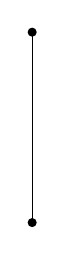
\begin{tikzpicture}[baseline={([yshift=-0.4ex]current bounding box.center)}]
      \begin{feynman}[inline=(a)]
        \vertex (a);
        \vertex (b);
        \diagram {
          a [dot] -- b [dot],
        };
        % \vertex [below=0.2em of a] {\(_{x}\)};  
        % \vertex [below=0.2em of b] {\(_{y}\)};  
      \end{feynman}
    \end{tikzpicture} = \frac{i}{2}
    \int d^Dz_1\, d^Dz_2\, J(z_1) \Delta(z_1-z_2) J(z_2) \, .
\end{equation}
Taking the functional derivatives with respect to $J$ we get a factor
of two, from acting with each derivative on both $J(z_1)$ and
$J(z_2)$:
\begin{equation}
  \label{eq:2ptOrderZeroTwo}
  G^{(2,0)}(x,y) = \frac{1}{i} \Delta(x-y)\, ,
\end{equation}
where the second index in the suffix indicates the order in the
perturbative expansion as discussed above. 

\noindent
It is easy to verify that there are no contributions to $Z[J]$ with
$E=2$ and $V=1$. 

\paragraph{V=2}

The next contributions to the two-point functions
come from terms with $V=2$, and there are two distinct diagram
topologies at this order.
\begin{enumerate}
\item [a.] The first diagram topology that contributes to $G^{(2)}$ is
  \begin{align}
    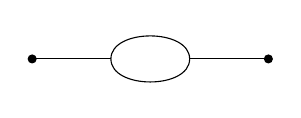
\begin{tikzpicture}[baseline={([yshift=-0.4ex]current bounding box.center)}]
      \begin{feynman}[inline=(a)]
        \vertex (a);
        \vertex (v1); 
        \vertex (v2); 
        \vertex (b);
        \diagram* {
          a [dot] -- v1 -- [out=90, in=90] v2 -- b [dot],
          v1 -- [out=-90, in=-90]  v2,
        };
      \end{feynman}
    \end{tikzpicture} = &\frac{1}{2^2} \int d^Dz_1\, d^Dz_2\, d^Dw_1\,
      d^Dw_2\, \times \nonumber \\
    &  \times J(z_1) \Delta(z_1-w_1) \Delta(w_1-w_2)^2 \Delta(w_2-z_2) J(z_2)\, .
  \end{align}
  Taking derivatives and inserting the appropriate factor of $i$
  yields a total contribution of
  \begin{align}
    G^{(2,2)}_a(x,y) = - \frac{1}{2} 
    \int d^Dw_1\, d^Dw_2\, \Delta(x-w_1) \Delta(w_1-w_2)^2
    \Delta(w_2-y)\, .
  \end{align}

\item [b.] The other contribution comes from 
  \begin{align}
    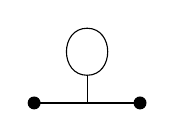
\begin{tikzpicture}[baseline={([yshift=-2.95ex]current bounding box.center)}]
      \begin{feynman}[vertical'=i to c]
        \vertex (c);
        \vertex [left=1.7em of c, dot] (a) {}; 
        \vertex [dot, right=1.7em of c](b) {};
        \vertex [above=1.0em of c](i);
%      \vertex (j);
 %     \vertex (k);
      \vertex [above=1.7em of i] (m);
      \diagram* {
%        j -- [draw=none]  i -- [draw=none] k, 
        (i) -- [half left] (m) -- [half left] (i),
%        i -- [out=155, in=25, loop, min distance=3cm] i,
        (a) -- (c) -- (b), 
        (c) -- (i), 
      };
%       \vertex [below=0.2em of a] {\(_{i_1}\)};  
%       \vertex [below=0.2em of b] {\(_{i_2}\)};  
% %      \vertex [below=0.2em of c] {\(c\)};  
%       \vertex [below=0.2em of i] {\(_{i}\)};  
    \end{feynman}
    % \begin{feynman}
    %     \vertex (v1);
    %     \vertex [left=of v1] (a); 
    %     \vertex [above=of v1] (v2); 
    %     \vertex [right=of v1] (b);
    %     \diagram* {
    %       (a) -- (v1)-- (b),
    %       (v1) -- (v2) -- [out=135, in=45, loop, min distance=3cm]  (v2),
    %     };
    %   \end{feynman}
    \end{tikzpicture} = &\frac{1}{2^2} \int d^Dz_1\, d^Dz_2\, d^Dw_1\,
      d^Dw_2\, \times \nonumber \\
    &  \times J(z_1) \Delta(z_1-w_1) \Delta(w_1-z_2) \Delta(w_1-w_2)
      \Delta(0) J(z_2)\, .
  \end{align}
  The net contribution from this diagram is
  \begin{align}
     G^{(2,2)}_b(x,y) = -\frac{1}{2} 
    \int d^Dw_1\, d^Dw_2\, \Delta(x-w_1) \Delta(w_1-y) \Delta(w_1-w_2)
      \Delta(0))\, .
  \end{align}
\end{enumerate}

\subsection{Momentum space}
\label{sec:momentum-space}

It is useful to write this correlators in momentum space. We already
discussed the representation of the free propagator in momentum space: 
\begin{align}
  \Delta(x) = \int \frac{d^Dp}{(2\pi)^D}\, e^{-ip\cdot x}
  \frac{1}{p^2 - m^2 + i\epsilon}\, .
\end{align}
The Fourier transform of the two-point correlator is defined as
\begin{align}
  \tilde{G}^{2}\left(p,p'\right) 
  &= 
    \int d^Dx\, d^Dy\, e^{ip\cdot x} e^{ip'\cdot y} 
    G^{(2)}(x,y) \\
  &= \int d^Dz\, d^Dy\, e^{ip\cdot z} e^{i(p+p')\cdot y} G^{(2)}(z) \\
  &= \left(2\pi\right)^D \delta(p+p')\, \int d^Dz\, e^{ip\cdot z}
    G^{(2)}(z)  \\
  &= \left(2\pi\right)^D \delta(p+p')\, \frac{1}{i} \tilde{\Delta}_F(p)\, .
\end{align}
Note that translation invariance of $G^{(2)}(x,y)$ produces an overall
Dirac delta that implements conservation of the total momentum. Again
we can look at the contributions to $\tilde{G}^{(2)}(p,p')$ order by
order in perturbation theory. 

\paragraph{V=0}

At lowest order in $g$, we simply have the Fourier transform of the
free propagator:
\begin{align}
  \tilde{G}^{(2,0)}(p,p') 
  &= 
    \left(2\pi\right)^D \delta(p+p')\,
    \frac{1}{i} \tilde{\Delta}(p) \\
  &=
    \left(2\pi\right)^D \delta(p+p')\,
    \frac{1}{i} \frac{1}{p^2-m^2+i\epsilon}\, .
\end{align}

\paragraph{V=2}

At order $g^2$, we obtain
\begin{align}
  \tilde{G}^{(2,2)}_a(p,p') 
  =& - \frac12\, \left(2\pi\right)^D \delta(p+p')\,
     \frac{1}{p^2-m^2+i\epsilon} \times \nonumber \\
   & \times \left\{
     \int \frac{d^D\ell}{(2\pi)^D}\, 
     \frac{1}{\ell^2-m^2+i\epsilon}
     \frac{1}{(\ell-p)^2-m^2+i\epsilon}
     \right\}
     \frac{1}{p^2-m^2+i\epsilon} \, .
\end{align}
The above expression can be represented by a Feynman diagram in
momentum space:
\begin{equation}
  \begin{tikzpicture}%[baseline=\plusheight]
    \begin{feynman}
      \vertex (a);
      \vertex [left=0.7cm of a] (i1);
      \vertex [right= of a] (b);
      \vertex [right=0.7cm of b] (f1);
      \diagram [horizontal=a to b, layered layout] {
        (i1) -- [momentum={\(p\)}] (a)
        -- [half left, momentum={[arrow shorten=0.4]\(\ell\)}] (b) 
        -- [half left, momentum={[arrow shorten=0.35]\(\ell-p\)}] (a) ,
        (f1) -- [momentum'=\(p'\)] (b)
      };
    \end{feynman}
  \end{tikzpicture}
\end{equation}
The Feynman rules in momentum space can be summarised as follows
(adapted from Srednicki's book). 
\begin{enumerate}
\item Draw $n$ lines for a $n$-point correlator. 
\item Leave one end of each external line free, and attach the other
  to the lines coming out of a vertex. 
\item The $i$-th external line carries momentum $p_i$, which we assume
  to be incoming momentum, and represent with a line pointing towards
  the vertex.
\item Four-momenta flow along the arrows, and the total momentum is
  conserved at each vertex. For a diagram without loops, this fixes
  the momentum of \emph{all} internal lines. 
\item The value of the diagram is given by the product of a factor of
  $i/(p^2-m^2+i\epsilon)$ for each line with momentum $p$, a factor of
  $1/i$ for the external end of a line, and a factor $ig (1/i)^\#$ for
  each vertex, where $\#$ is the number of legs connecting at each
  vertex. 
\item A diagram with $L$ loops will have $L$ internal momenta that are
  not fixed by momentum conservation. We integrate over those momenta,
  with measure $d^p/(2\pi)^D$. 
\item Determine the symmetry factor associated to permutations of
  \emph{internal} propagators and vertices. 
\end{enumerate}

\begin{Ex}
  Use the Feynman rules in momentum space to compute
  $G^{(2,2)}_b$. Check that you get the same result by performing a
  Fourier transform of the result in position space.
\end{Ex}

\section{Physical states}
\label{sec:physical-states}

The eigenstates of the Hamiltonian form a complete set of states. They
can be classified in three categories.
\begin{enumerate}
\item The vacuum state $\ket{0}$ is the lowest energy state, and
  corresponds to a state with no particles.
\item The one-particle states $|\mathbf{p},\sigma\rangle$ are
  classified by their spatial momentum. Their energy is given by the
  relativistic dispersion relation 
  \begin{equation}
    \label{eq:RelDispRel}
    E_p = \sqrt{\mathbf{p}^2 + \mphys^2}\, ,
  \end{equation}
  where $\mphys$ denotes the physical mass of the state. Note that the
  physical mass \emph{does not} need to coincide with the mass that
  appears in the Lagrangian. We will discuss this point in detail
  later. Any other quantum number necessary to identify the particle
  is denoted here by $\sigma$.  The states are normalised by imposing
\begin{equation}
  \label{eq:OnePartNorm}
  \langle \mathbf{p}, \sigma | \mathbf{p}', \sigma' \rangle =
  \delta_{\sigma\sigma'}\, 
  2 E_p\, (2\pi)^{D-1} \delta(\mathbf{p}-\mathbf{p}')\, .
\end{equation}
\item The multiparticle states $|\mathbf{P};n\rangle$ are classified
  by their total spatial momentum $\mathbf{P}$, plus other parameters
  such as the relative momenta between the particles, which we denote
  collectively by $n$. The energy of the mutiparticle states is
  $\sqrt{\mathbf{P}^2+M^2}$, where $M^2$ is one of the parameters
  included in $n$. The threshold for producing multiparticle states is
  given by the energy of two particles at rest $M=2\mphys$.
\end{enumerate}
The completeness relation can be written as
\begin{align}
  \ketbra{0}{0}
  &+ \sum_\sigma \int d\Omega_p 
    |\mathbf{p},\sigma\rangle \langle \mathbf{p},\sigma| + \nonumber
  \\
  &+ \sum_n \int d\Omega_P 
    |\mathbf{P},n\rangle \langle \mathbf{P},n|\, = 1\, ,
\end{align}
and we have introduced the Lorentz-invariant integration measure
\begin{align}
  d\Omega_p = \frac{d^{D-1}p}{(2\pi)^{D-1}}
    \frac{1}{2E_p} \, .
\end{align}
Note that the 'sum' over $n$ is a short-hand notation, which may
involve integrations over continuum variables such as the relative
momentum, or the invariant mass of the state. 

\section{Polology}
\label{sec:polology}

In this section, we shall learn some features about the analytic
structure of field correlators, and discuss their relevance in order
to extract physical information from the correlators. Starting from an
$n$-point correlator in momentum space,
\begin{align}
  \tilde{G}^{(n)}\left(p_1, \ldots, p_n\right) 
  = \int d^Dx_1\, \ldots d^Dx_n\, 
  e^{-i p_1\cdot x_1} \ldots e^{-i p_n\cdot x_n}\, 
  \langle T\phi(x_1) \ldots \phi(x_n)\rangle\, ,
\end{align}
we want to focus on the contribution coming from the sector where the
values $x_1^0, \ldots, x_r^0$ are all larger than the values of
$x_{r+1}^0, \ldots, x_n^0$, for some value of $r$ between 1 and
$n-1$. This contribution can be written as 
\begin{align}
  \tilde{G}^{(n)}\left(p_1, \ldots, p_n\right) 
  =& \int d^Dx_1\, \ldots d^Dx_n\, 
  e^{-i p_1\cdot x_1} \ldots e^{-i p_n\cdot x_n}\, \times \nonumber \\
   &\times \theta\left(
     \min\{x_1^0 \ldots x_r^0\} - \max\{x_{r+1}^0 \ldots x_n^0\}
     \right) \nonumber \\
   &\times \langle T\Big[\phi(x_1) \ldots \phi(x_r)\Big]
     T\Big[\phi(x_{r+1}) \ldots \phi(x_n)\Big]
     \rangle\, .
\end{align}
We can introduce a complete set of states in-between the two
$T$-ordered products, and look at the result coming from the
one-particle states. Defining new integration variables
\begin{align}
  x_i = x_1 + y_i\, , \quad \mathrm{for}\ i=2, \ldots, r\, ,
\end{align}
we can write
\begin{align}
  \phi(x_1) \ldots \phi(x_r) 
  &= \phi(x_1) \ldots \phi(x_1+y_i) \ldots \phi(x_1+y_r) \nonumber \\
  &= e^{i P\cdot x_1} \phi(0) e^{-i P\cdot x_1} \ldots e^{i P\cdot
    x_1} \phi(y_i) e^{-i P\cdot x_1} \ldots e^{i P\cdot x_1} \phi(y_r)
    e^{-i P\cdot x_1}\, ,
\end{align}
and hence
\begin{align}
  \bra{0} T \phi(x_1) \ldots \phi(x_r) | p,\sigma\rangle = 
  e^{-i p \cdot x_1}  \bra{0} T \phi(0) \ldots \phi(y_r) |
  p,\sigma\rangle\, .
\end{align}
A similar shift of the integration variables can be done using
\begin{align}
  x_i = x_{r+1} + y_i\, , \quad \mathrm{for}\ i=r+2, \ldots, n\, ,
\end{align}
The argument of the theta function can be rewritten as
\begin{align}
  \min\{x_1^0 \ldots x_r^0\} - \max\{x_{r+1}^0 \ldots x_n^0\} = 
  x_1^0 -x_{r+1}^0 + \min\{0 \ldots y_r^0\} - \max\{0 \ldots y_n^0\}\, .
\end{align}
Using the integral representation of the theta,
\begin{align}
  \theta(\tau) = -\frac{1}{2\pi i} \int_{-\infty}^{+\infty} d\omega\,
  \frac{e^{-i\omega \tau}}{\omega + i\epsilon}\, ,
\end{align}
and performing the integrals over $x_1$ and $x_{r+1}$, yields
\begin{align}
  \tilde{G}^{(n)}(p_1, \ldots, p_n) 
  &= \int d^Dy_2 \ldots d^Dy_r\, d^Dy_{r+2} \ldots d^Dy_n \, \nonumber
  \\
  & \times e^{-ip_2\cdot y_2} \ldots e^{-ip_{r}\cdot y_r} 
    \, e^{-ip_{r+2}\cdot y_{r+2}} \ldots e^{-ip_{n}\cdot y_n}
    \nonumber \\
  & \times \frac{-1}{2\pi i} \int \frac{d\omega}{\omega + i\epsilon}\, 
    \exp\left\{
    -i \omega \left[ 
    \min\{0 \ldots y_r^0\} - \max\{0 \ldots y_n^0\}
    \right]
    \right\} \nonumber \\
  & \times \sum_\sigma \int d\Omega_p
    \bra{0}  T \phi(0) \ldots \phi(y_r) |
    p,\sigma\rangle \langle p, \sigma | T \phi(0) \ldots \phi(y_n)
    \ket{0} \nonumber \\
  & \times (2\pi)^D \delta(\mathbf{p} - \mathbf{p}_1 - \ldots -
    \mathbf{p}_r) \, 
    \delta(E_p + \omega - p_1^0 - \ldots - p_{r}^0) \nonumber \\
  & \times (2\pi)^D \delta(\mathbf{p} + \mathbf{p}_{r+1} + \ldots +
    \mathbf{p}_n) \, 
    \delta(E_p + \omega + p_{r+1}^0 + \ldots + p_{n}^0) \, .
\end{align}
Performing the integrals over the spatial components of $p$ and
$\omega$ yields
\begin{align}
  &\delta(\mathbf{p}_1+ \ldots +\mathbf{p}_n)\, \mathrm{and}\, , \nonumber \\
  & \delta(p_1^0 + \ldots + p_n^0) \frac{1}{q^0-E_p +i\epsilon}\, ,
\end{align}
respectively, where the four-momentum $q$ is defined as
\begin{align}
  q=p_1 + \ldots + p_r = -p_{r+1} - \ldots - p_n\, .
\end{align}
Finally, if we are interested in the residue at the pole, we can rewrite
\begin{align}
  \frac{1}{q^0-E_p + i\epsilon} \longrightarrow \frac{2 E_p}{q^2-\mphys^2 + i\epsilon}\, 
\end{align}
Collecting all the terms, and ignoring a phase factor that reduces to
one at the pole, we find that the one-particle state contribution to the
integration over the specific sector that we considered above yields
\begin{align}
  \tilde{G}^{(n)}(p_1,\ldots,p_n) \longrightarrow
  \delta(p_1+\ldots+p_n)\, \frac{1}{q^2-\mphys^2+i\epsilon}\, 
  \sum_\sigma M_{0|q\sigma}(p_2,\ldots,p_r) M_{q\sigma|0}(p_{r+2},
  \ldots, p_n)\, .
\end{align}
In the equation above we have defined
\begin{align}
  M_{0|q\sigma}(p_2,\ldots,p_r) 
  &= \int d^Dy_2 \ldots d^Dy_r\, 
    e^{-ip_2\cdot y_2} \ldots e^{-ip_r\cdot y_r}
    \mel{0}{T \phi(0) \ldots \phi(y_r)}{q,\sigma}, \\
 M_{q\sigma|0}(p_{r+2},\ldots, p_n) 
  &= \int d^Dy_{r+2} \ldots d^Dy_n\, 
    e^{-ip_{r+2}\cdot y_{r+2}} \ldots e^{-ip_n\cdot y_n}
    \mel{q,\sigma}{  T \phi(0) \ldots \phi(y_n)}{0},
\end{align}
and we notice that this contribution appears multiplied by a Dirac
delta that enforces the conservation of total momentum. The important
result here is that the correlators in momentum space have a pole
singularity whenever $q=p_1+\ldots+p_r$ \emph{goes on-shell}, \ie
$q^2=\mphys^2$.

Note that these results are completely general, and in particular do
not rely on the perturbative definition of the correlators. 

\section{Källén-Lehmann representation}
\label{sec:kall-lehm-repr}

Let us now come back to the 2-point function, and find a representation
that allows us to extract some physical information about the scalar
field. We define the full propagator as
\begin{equation}
  \label{eq:FullProp}
  \Delta_F(x-y) = i \bra{0} T \phi(x) \phi(y) \ket{0} \, ,
\end{equation}
and define the field so that
\begin{equation}
  \label{eq:FieldNorm}
  \bra{0} \phi(x) \ket{0} = 0\, ,\ \mathrm{and}\
  \langle \mathbf{p}| \phi(0) \ket{0} = 1\, ,
\end{equation}
where $\ket{\mathbf{p}}$ represents the physical one-particle state,
and we have dropped the dependence on $\sigma$. As usual the full
propagator in momentum space is defined by taking the Fourier
transform:
\begin{equation}
  \label{eq:FullPropMom}
  \tilde{\Delta}_F(p) = 
  \int d^Dx\,  e^{ip\cdot(x-y)} \Delta(x-y)\, .
\end{equation}

\paragraph{Free theory}

With these conventions, the free theory result for the propagator is
\begin{equation}
  \label{eq:FreePropAgain}
  \tilde\Delta(p) = \frac{1}{p^2-m^2+i\epsilon}\, .
\end{equation}
Eq.~(\ref{eq:FreePropAgain}) shows that $\tilde{\Delta}$ has a pole at
$p^2=m^2$. For the free particle we find a pole in the propagator,
at a value which coincides with the parameter in the Lagrangian.

\paragraph{Interacting theory}

For the interacting theory, we can derive a general expression, which
again does not rely on the perturbative definition of the two-point
function. Let us first consider the case where $x^0>y^0$:
\begin{align}
  \bra{0} T \phi(x) \phi(y) \ket{0}
  =& \bra{0} \phi(x) \phi(y) \ket{0} \nonumber \\
  =& \bra{0} \phi(x) \ket{0} \bra{0} \phi(y) \ket{0} +
     \nonumber \\
  &+ \int d\Omega_p\, \bra{0} \phi(x)| \mathbf{p}\rangle
    \langle \mathbf{p} | \phi(y) \ket{0} + \nonumber \\
  &+ \sum_n \int d\Omega_P\, \bra{0} \phi(x) |\mathbf{P}, n\rangle
    \langle \mathbf{P}, n |\phi(y) \ket{0}\, .
\end{align}
The conventions in Eq.~(\ref{eq:FieldNorm}) allow us to simplify the
expression above.
\begin{align}
  \bra{0} T \phi(x) \phi(y) \ket{0}
  =& \int d\Omega_p\, e^{-ip\cdot (x-y)} + \nonumber \\
   &+ \sum_n \int d\Omega_p\, e^{-ip\cdot (x-y)}\, \left|
    \langle \mathbf{p}, n |\phi(0) \ket{0} \right|^2 \, .
\end{align}
Because we are working with a scalar field, the matrix element
$\langle \mathbf{p}, n |\phi(0) \ket{0}$ is invariant under Lorentz
transformations, and therefore can only depend on $p$ via the
invariant mass $M^2$. We can therefore introduce the \emph{spectral
  density}
\begin{align}
  \label{eq:SpecDen}
  \rho(s) = \sum_n \left|
    \langle \mathbf{p}, n |\phi(0) \ket{0} \right|^2 \, 
  \delta(s-M^2)\, ,
\end{align}
and write the two-point correlator as
\begin{align}
  \bra{0} T \phi(x) \phi(y) \ket{0}
  =& \int d\Omega_p\, e^{-ip\cdot (x-y)} + \nonumber \\
   &+ \int_{4m^2}^\infty ds\, \rho(s) \int d\Omega_p\,  e^{-ip\cdot
     (x-y)}\, .
\end{align}
Similar manipulations for the case $y^0>x^0$ yield
\begin{align}
  \bra{0} T \phi(x) \phi(y) \ket{0}
  =& \int d\Omega_p\, e^{ip\cdot (x-y)} + \nonumber \\
   &+ \int_{4m^2}^\infty ds\, \rho(s) \int d\Omega_p\,  e^{ip\cdot
     (x-y)}\, .
\end{align}
Collecting both contributions to the $T$-ordered product 
\begin{align}
  \bra{0} T \phi(x) \phi(y) \ket{0}
  = \theta(x^0-y^0)  \bra{0} \phi(x) \phi(y) \ket{0}
  + \theta(y^0-x^0)  \bra{0} \phi(y) \phi(x) \ket{0}\, ,
\end{align}
and using 
\begin{align}
  \frac{1}{i} \int \frac{d^Dp}{(2\pi)^D}\,
  \frac{e^{-ip\cdot(x-y)}}{p^2-\mphys^2+i\epsilon} = 
  \theta(x^0-y^0) \int d\Omega_p\, e^{-ip\cdot(x-y)} +
  \theta(y^0-x^0) \int d\Omega_p\, e^{ip\cdot(x-y)}\, , 
\end{align}
we finally obtain
\begin{align}
  \bra{0} T \phi(x) \phi(y) \ket{0}
  =& \int \frac{d^Dp}{(2\pi)^D}\,
     e^{-ip\cdot(x-y)} \Big[
     \frac{1}{p^2-\mphys^2+i\epsilon} + \nonumber \\
  \label{eq:KLFourier}
  & + \int_{4\mphys^2}^\infty ds\, \rho(s) \frac{1}{p^2-s+i\epsilon} 
     \Big]\, .
\end{align}
Eq.~(\ref{eq:KLFourier}) allows us to read the expression for the full
propagator in momentum space:
\begin{align}
  \label{eq:KLusual}
  \tilde{\Delta}_F(p) = \frac{1}{p^2-\mphys^2+i\epsilon} 
  + \int_{4\mphys^2}^\infty ds\, \rho(s) \frac{1}{p^2-s+i\epsilon}\, . 
\end{align}
We see that the two-point correlator of a field $\phi$ that satisfies
the conditions in Eq.~(\ref{eq:FieldNorm}) has a pole for
$p^2=\mphys^2$, with residue exactly equal to one. Note that the field
$\phi$ does not need to be the field that appears in the
Lagrangian. Knowledge about the multiparticle states of the theory is
encoded in the two-point function via the integral on the RHS side of
Eq.~(\ref{eq:KLusual}). 

\section{S Matrix}
\label{sec:s-matrix}

In order to compute the quantum amplitude for a physical process
involving arbitrary numbers of particles in the initial and final
state, we need to compute the overlap of a state prepared in the
distant past (the so-called \emph{in} state), with the resulting final
state in the distant future (the so-called \emph{out} state). If
we want to describe a $2\to n$ process -- like a $pp$ collision at
the LHC -- we need to compute
\begin{equation}
  \label{eq:ScattAmpl}
  \langle \mathbf{p}_1, \ldots, \mathbf{p}_n; \mathrm{out} |
  \mathbf{k}_1, \mathbf{k}_2; \mathrm{in}\rangle\, .
\end{equation}
The $S$-matrix allows us to express this scalar product between in-
and out-states in terms of states defined at any common reference
time: 
\begin{equation}
  \label{eq:SMatDef}
   \langle \mathbf{p}_1, \ldots, \mathbf{p}_n; \mathrm{out} |
  \mathbf{k}_1, \mathbf{k}_2; \mathrm{in}\rangle = 
   \langle \mathbf{p}_1, \ldots, \mathbf{p}_n | S |
  \mathbf{k}_1, \mathbf{k}_2\rangle\, .
\end{equation}
It is usual to separate the $S$ matrix into the identity operator,
corresponding to particles not interacting, plus a non-trivial part
which is usually denoted $T$:
\begin{equation}
  \label{eq:TMatDef}
  S = 1 + i T\, .
\end{equation}

\section{LSZ reduction}
\label{sec:lsz-reduction}

An important corollary of the result shown in
section~\ref{sec:polology} is obtained by setting $r=1$. In this case,
the previous discussion allows us to conclude that the correlators in
momentum space have a pole whenever the momentum of one of the fields
is on-shell. Therefore an $n$-point correlation function has (at
least) $n$ poles, each corresponding to one of the momenta
$p_i\to \mphys^2$. The residue at this multiple pole yields the $S$-matrix
for a scattering process involving $n$-particles:
\begin{align}
   \braket{ p_{1}' \ldots p_{m'}'; \mathrm{out} }{ p_{1} \ldots p_{m};
  \mathrm{in}}
  =& 
  \mel{p_{1}' \ldots p_{m'}'}{S}{p_{1} \ldots p_{m}} \\
  =& 
  \lim_{p_j^2,p_k'^2 \to \mphys^2} \prod_{k=1}^{m'}
  (p_k'^2-\mphys^2+i\epsilon)
  \prod_{j=1}^{m}
  (p_j^2-\mphys^2+i\epsilon) \, \nonumber \\
  & \times 
    \tilde{G}^{(m+m')}(p_1, \ldots, p_{m}, -p_1', \ldots, -p_{m'}')\, ,
\end{align}
where $n=m+m'$, and the fields are normalised so that
\begin{align}
  \langle \mathbf{p} | \phi(0) \ket{0} = 1\,.
\end{align}
We will return to the question of the normalisation of the field
later. The LSZ reduction formula provides an elegant way to represent
quantum amplitudes using Feynman diagrams in momentum space. We adopt
the same rules discussed above, with the following modifications.
\begin{enumerate}
\item We associate an outgoing momentum to the external lines that
  correspond to particles in the final state. 
\item We multiply each external line by a factor of
  $-i(p^2-\mphys^2+i\epsilon)$ -- the correlators multiplied by these
  factors are called \emph{truncated} (or \emph{amputated}) correlators.
\end{enumerate}

A heuristic derivation of the LSZ reduction formula is discussed in
Problem Sheet 4.

\begin{Ex}
  Compute the amplitude for the scattering process
  \[
    p_1 p_2 \longrightarrow p_1' p_2'
  \]
  at order $g^2$ in the $\phi^3$ scalar theory. You can assume that
  $\mphys=m$ in this calculation.
\end{Ex}

\section{Optical Theorem}
\label{sec:optical-theorem}

Physical constraints translate into relations between correlators. It
is important to be able to derive these relations, and to understand
their physical content. One example is provided by the unitarity of
the $S$-matrix, \ie by the conservation of probability in quantum
mechanics. Unitarity is written as
\begin{equation}
  \label{eq:SmatUnit}
  S^\dagger S = 1\, .
\end{equation}
Inserting the representation of $S$ in terms of the transition matrix
yields
\begin{equation}
  \label{eq:TmaUnit}
  -i \left(T - T^\dagger\right) = T^\dagger T\, .
\end{equation}
Let us consider the matrix element of Eq.~(\ref{eq:TmaUnit}) between an
initial state $a$ and a final state $b$, and let us factor out a Dirac
delta that corresponds to total momentum conservation, 
\begin{equation}
  \label{eq:MAmplitude}
  \bra{b} T \ket{a} = (2\pi)^D \delta(P_a - P_b)\, \mathcal{M}(a
  \to b)\, .
\end{equation}
Some simple algebra yields on the LHS
\begin{equation}
  \label{eq:MLHS}
  -i (2\pi)^D \delta\left(P_a-P_b\right) \left[
    \mathcal{M}(a\to b) - \mathcal{M}(b \to a)^*
    \right]\, . 
\end{equation}
On the RHS we can insert a complete set of states, and rewrite it as
\begin{equation}
  \label{eq:MRHS}
   (2\pi)^D \delta\left(P_a-P_b\right) \sum_f \int d\Omega_f\,
   (2\pi)^D \delta\left(P_a-P_f\right) \mathcal{M}(b\to f)^*
   \mathcal{M}(a\to f)\, .
 \end{equation}
The unitarity condition simplifies for $a=b$, 
\begin{equation}
  \label{eq:OptThm}
  2 \mathrm{Im}\ \mathcal{M}(a\to a) = 
  \sum_f \int d\Omega_f  (2\pi)^D \delta\left(P_a-P_f\right) 
  \left|
    \mathcal{M}(a\to f)
  \right|^2\, .
\end{equation}
This is the so-called \emph{optical theorem}, which relates the
imaginary part of the forward $a\to a$ amplitude (LHS) to the total cross
section $a\to f$ (RHS), summed over \emph{all} final states $f$.

\section{Ward identities}
\label{sec:ward-identities}

The final example of relations between correlators that we are going
to discuss are the so-called \emph{Ward identities}. Ward identities
are equalities between field correlators that are obtained as a
consequence of symmetries of the system. In classical mechanics,
symmetries of the action translate into conserved currents according
to Noether's theorem. As we will show in this section, the analogue of
current conservation in quantum field theory is precisely the Ward
identity. 

In order to derive the identities, let us start by considering a
symmetry transformation of the field, \ie a transformation
\begin{equation}
  \label{eq:FieldTrans}
  \phi(x) \mapsto \phi'(x)=\phi(x) + \epsilon \delta\phi(x) \, ,
\end{equation}
such that for constant $\epsilon$ the action is unchanged. If we introduce
a dependence on the space-time coordinate, $\epsilon(x)$, then the
variation of the action can be written
\begin{align}
  \label{eq:SVar}
  \delta S &= \int d^Dx\, \frac{\delta S}{\delta\phi(x)} \epsilon(x)
             \delta\phi(x) \\
             &= -\int d^Dx\, \epsilon(x) \partial_\mu j^\mu(x)\, , 
\end{align}
where $j^\mu(x)$ is precisely the Noether current that is conserved in
the classical theory. 

In order to derive the Ward identities, we use
Eq.~(\ref{eq:FieldTrans}) to perform a change of integration variables
in the functional integral
\begin{equation}
  \label{eq:ChangeOfVars}
  \int \mathcal{D}\phi\, e^{iS[\phi]} O(\phi) = 
  \int \mathcal{D}\phi'\, e^{iS[\phi']} O(\phi') \, ,
\end{equation}
and then expand the RHS to first order in $\epsilon$:
\begin{align}
  \int \mathcal{D}\phi\, e^{iS[\phi]} O(\phi) 
  =& \int \mathcal{D}\phi\, e^{iS[\phi]}\, 
     \left[
     1 + i \delta S[\phi]
     \right]\, 
     \left[
     O(\phi) + \delta O
     \right]
     \, ,
\end{align}
where $O$ is a generic function of the field $\phi$. We can now
substitute the expressions for $\delta S$ and $\delta O$:
\begin{align}
  \int \mathcal{D}\phi\, e^{iS[\phi]} \left\{
  -i \int d^Dx\, \epsilon(x) \partial_\mu j^\mu(x)
  O(\phi) + \int d^Dx\, \frac{\delta O(\phi)}{\delta\phi(x)} \epsilon(x)
  \delta \phi(x)
  \right\} = 0\, .
\end{align}
Rearranging the terms above allows us to write the identity in a way
that makes its physical content more obvious: 
\begin{align}
  \label{eq:IntWardId}
  \int d^Dx\, \epsilon(x) \left\{
  -i \langle \partial_\mu j^\mu(x)
  O(\phi) \rangle +  
  \langle \frac{\delta O(\phi)}{\delta\phi(x)}
  \delta \phi(x) \rangle \right\} = 0\, .
\end{align}
Eq.~(\ref{eq:IntWardId}) is sometimes referred to as an {\em
  integrated Ward identity}. Since it has to be satisfied for every
function $\epsilon(x)$, we can derive the \emph{Ward identity}:
\begin{align}
  \label{eq:WardId}
   -i \langle \partial_\mu j^\mu(x)
  O(\phi) \rangle +  
  \langle \frac{\delta O(\phi)}{\delta\phi(x)}
  \delta \phi(x) \rangle = 0\, .
\end{align}
There are two important physical results encoded in Eq.~(\ref{eq:WardId}).
\begin{enumerate}
\item Symmetry in QFT translates into a relation between
  correlators. This is true beyond perturbation theory and is used in
  defining the renormalization conditions in QFT.
\item Current conservation in QFT is realised at the level of the
  insertion of $\partial_\mu j^\mu(x)$ in field correlators, up to
  the terms that come from the variation of $O$. If $O$ is a product
  of local fields, this variations is localised in space-time, \ie the
  contributions are all proportional to Dirac deltas. These terms are
  called \emph{contact terms}.  
\end{enumerate}

Note that in deriving the Ward identity above we have assumed that the
integration measure $\mathcal{D}\phi$ is invariant, \ie
$\mathcal{D}\phi=\mathcal{D}\phi'$. There are examples where the
measure is \emph{not} invariant, which lead to extra terms in the Ward
identities. In these cases the Ward identities are called {\em
  anomalous}. 
\end{document}

\chapter{Path Integrals for Gauge Fields}
\label{cha:path-integrals-gauge}
% !TeX root = ./notes.tex

\documentclass[notes]{subfiles}

\renewcommand{\tphi}{\tilde{\phi}}
\renewcommand{\tj}{\tilde{J}}
\renewcommand{\tchi}{\tilde{\chi}}
\renewcommand{\psibar}{\bar{\psi}}
\renewcommand{\etabar}{\bar{\eta}}

\setcounter{chapter}{4}

\begin{document}
\chapter{Path Integrals for Fermion Fields}
\label{cha:path-integr-ferm}
\section{Fermion Path Integral}
\label{sec:ferm-path-integr}

For the case of fermion fields, we want to define the path integral
following the recipe we used for the scalar field. We will treat the
fields $\psi$ and $\bar\psi$ as Grassmann variables, \ie 
\begin{equation}
  \label{eq:GrassVar}
  \left\{\psi_\alpha(x),\psi_\beta(y)\right\}=0\, .
\end{equation}
In order to have a consistent implementation of the anticommuting
properties of the fermion fields, the functional derivative with
respect to a Grassmann variable must be a Grassmann variable
itself. As a consequence
\begin{equation}
  \label{eq:GrassDer}
  \frac{\delta^2 F}{\delta \psi_\alpha(x) \delta\psi_\beta(y)} = 
  -\frac{\delta^2 F}{\delta \psi _\beta(y) \delta\psi_\alpha(x)}\, ,
\end{equation}
and 
\begin{equation}
  \label{eq:GrassDer2}
    \frac{\delta^2 F}{\delta \psi_\alpha(x) \delta\psi_\alpha(x)} = 0\,.
\end{equation}
In the definition of the generating functional, we introduce
independent sources for $\psi$ and $\bar{\psi}$:
\begin{equation}
  \label{eq:SourceTerm}
  \int d^Dy\, \left[
    \bar{\eta}(y) \psi(y) + \bar{\psi}(y) \eta(y)
    \right]\, ,
\end{equation}
such that
\begin{align}
  \label{eq:GrassDerivOne}
  \frac{\delta}{\delta\eta(x)} &\int d^Dy\, \left[
    \bar{\eta}(y) \psi(y) + \bar{\psi}(y) \eta(y)
    \right] = - \psibar(x)\, \\
  \label{eq:GrassDerivTwo}
  \frac{\delta}{\delta\etabar(x)} &\int d^Dy\, \left[
    \bar{\eta}(y) \psi(y) + \bar{\psi}(y) \eta(y)
    \right] = \psi(x)\, .
\end{align}

\paragraph{Free theory}

The action for the free Dirac field is
\begin{equation}
  \label{eq:FreeDiracAction}
  S_0\left[\psi,\psibar\right] = 
  \int d^Dx\, \psibar(x) \left( i \slashed{\partial} -m \right)
  \psi(x)\, .
\end{equation}
 Using the rules above for the functional derivative, we can find the
 classical equation of motion, \ie Dirac's equation
 \begin{align}
   \frac{\delta}{\delta \psibar(x)} S_0\left[\psi,\psibar \right] = 0
   \quad \Longrightarrow \quad
   \left(i \slashed{\partial} - m\right)\psi(x) =0\, .
 \end{align}
By analogy with the scalar case, we can write the generating
functional for the free theory:
\begin{align}
  Z_0\left[\etabar, \eta\right] 
  &= \int \mathcal{D}\psi\, \mathcal{D}\psibar\, 
    \exp\left\{
    i \left( S_0[\psi,\psibar] + \etabar \cdot \psi +
    \psibar \cdot \eta\right)
    \right\} \\
  &= \exp \left[
    - \int d^Dx\, d^Dy\, \etabar(x) S(x-y) \eta(y)
    \right]\, .
\end{align}
The Feynman propagator for the Dirac field is
\begin{equation}
  \label{eq:DiracFeynProp}
  S(x-y) = \int_p e^{-i p\cdot(x-y)}\,
  \frac{i (\slashed{p}+m)}{p^2-m^2+i\epsilon}\, .
\end{equation}
Note that, just like in the case of the scalar field, the propagator
is the inverse of the quadratic term in the action. The propagator is
a $4\times 4$ matrix in spin space, which we can write explicitely:
\begin{align}
  \langle 0|& T \psi_\alpha(x) \psibar_\beta(y) |0 \rangle 
  = \nonumber \\ 
  \label{eq:DiracFeynPropAllIndices}
  &= S_{\alpha\beta}(x-y) = 
  \int_pe^{i p\cdot(x-y)}\,
  \frac{i \left(p_\mu \left(\gamma^\mu\right)_{\alpha\beta}+m\,
    \delta_{\alpha\beta}\right)}
  {p^2-m^2+i\epsilon}\, .
\end{align}
Because of the linear term in $p$ in the propagator the fermionic
propagator is not symmetric in its arguments, and will be denoted with
an arrow pointing from one end to the other:
  \begin{equation}
    \label{eq:SPropXYFeynDiag}
    S(x-y) = 
    \begin{tikzpicture}[baseline={([yshift=1.4ex]current bounding box.center)}]
      \begin{feynman}[inline=(a)]
        \vertex (a);
        \vertex (b);
        \diagram {
          a --[fermion] b,
        };
        \vertex [below=0.2em of a] {\(_{x}\)};  
        \vertex [below=0.2em of b] {\(_{y}\)};  
      \end{feynman}
    \end{tikzpicture}\, .
  \end{equation}

Correlators of fermion fields are computed by taking derivatives with
respect to the source fields
\begin{align}
  \langle 0 |& T \psi_{\alpha_1}(x_1) \ldots \psibar_{\beta_1}(y_1)
  \ldots |0\rangle_0  = \nonumber \\
   &=\frac{1}{i} \frac{\delta}{\delta\etabar_{\alpha_1}(x_1)} \ldots
  i \frac{\delta}{\delta\eta_{\beta_1}(y_1)}\, 
  \left. Z_0\left[\eta, \etabar\right] \right|_{\eta=\etabar=0}\, .
\end{align}

\paragraph{Interacting theory}

If the interactions are specified by a potential
$V\left(\psi,\psibar\right)$, the generating functional is defined as 
\begin{equation}
  \label{eq:InterGenFunc}
  Z\left[\eta,\etabar\right] \propto
  \exp\left[
    i \int d^Dx\, V\left( i \frac{\delta}{\delta\eta(x)}, 
    \frac{1}{i} \frac{\delta}{\delta\etabar(x)}\right)
  \right] \, 
  Z_0\left[\eta, \etabar \right]\, , 
\end{equation}
and the normalization is fixed by requiring
\begin{equation}
  \label{eq:ZNorm}
  Z[0,0] = 1\, .
\end{equation}
A double expansion in powers of the interaction, and in powers of the
number of propagators defines the interacting path integral, as we did
for the case of scalars. 

\begin{subappendices}
  
\section{Differentiation in Grassmann variables}
\label{sec:diff-grassm-vari}

\paragraph{Grassmann algebra}

A Grassmann algebra $\mathcal{A}$, over $\mathbb{R}$ or $\mathbb{C}$,
is constructed from a set of generators $\theta_i$ satisfying
\begin{equation}
  \label{eq:AntiCommGen}
  \theta_i \theta_j + \theta_j \theta_i = 0\, .
\end{equation}
Note that 
\begin{enumerate}
\item all elements are first degree polynomials in each generator; 
\item if the number of generators is finite and equal to $n$, the
  algebra is vector space of dimension $2^n$.
\end{enumerate}

\paragraph{Grassmannian parity}

Parity is defined as an automorphism on $\mathcal{A}$ is defined by
\begin{equation}
  \label{eq:GrassParity}
  P(\theta_i) = - \theta_i\, .
\end{equation}
The action of $P$ on a monomial is
\begin{equation}
  \label{eq:GrassParMon}
  P(\theta_{i_1} \ldots \theta_{i_p}) = (-)^p \theta_{i_1} \ldots
  \theta_{i_p}\, .
\end{equation}
The reflection defines two eigenspaces containing the even and odd
elements:
\begin{equation}
  \label{eq:ParitySubspaces}
  P(\mathcal{A}^\pm) = \pm \mathcal{A}^\pm\, .
\end{equation}

\paragraph{Grassmann differentiation}

Differentiation is defined as a linear mapping
\begin{equation}
  \label{eq:GrassDiff}
  D: \mathcal{A} \to \mathcal{A}\, ,
\end{equation}
which satisfies
\begin{equation}
  \label{eq:GrassDiffProp}
  D(A_1 A_2) = P(A_1) D(A_2) + D(A_1) A_2\, ,
\end{equation}
which guarantees that
\begin{equation}
  \label{eq:GrassDiffParity}
  D P + P D = 0\, .
\end{equation}
Note that the image of $\mathcal{A}^\pm$ belongs to
$\mathcal{A}^\mp$, \ie derivation changes the parity of product of
Grassmann variables. 

We can introduce the nilpotent differential operators
$\partial/\partial\theta_i$ by
\begin{equation}
  \label{eq:DiffOpsBasis}
  \frac{\partial}{\partial \theta_i} \theta_j = \delta_{ij}\, . 
\end{equation}
The differential operators and the generators can be considered as
operators acting on the elements of $\mathcal{A}$ from the left. They
satisfy the anticommutation relations:
\begin{align}
  \label{eq:AntiComm1}
  \theta_i \theta_j + \theta_j \theta_i &= 0\, ,\\
  \label{eq:AntiComm2}
  \frac{\partial}{\partial\theta_i} \frac{\partial}{\partial\theta_j}
  + \frac{\partial}{\partial\theta_j}
  \frac{\partial}{\partial\theta_i} &= 0\, , \\
  \label{eq:AntiComm3}
  \theta_i \frac{\partial}{\partial\theta_j} +
  \frac{\partial}{\partial\theta_j} \theta_i &= 0\, .
\end{align}

\paragraph{Chain rule}

If $\sigma(\theta)\in\mathcal{A}^-$, $x(\theta)\in \mathcal{A}^+$,
then
\begin{equation}
  \label{eq:GrassChainRule}
  \frac{\partial}{\partial\theta} f(\sigma,x) = 
  \frac{\partial\sigma}{\partial\theta} \frac{\partial
    f}{\partial\sigma} 
  + \frac{\partial x}{\partial\theta} \frac{\partial f}{\partial x}\, .
\end{equation}

\section{Integration in Grassmann variables}
\label{sec:integr-grassm-vari}

To a given differential operator $D$ we associate an integral
operator $I$. The idea is to generalise the concept of {\em definite}
integral to the case of Grassmann variables. $I$ is defined by
requiring a number of properties that are {\em expected} to hold for
an integral. 
\begin{enumerate}
\item $I$ is linear
  \begin{equation}
    \label{eq:LinearGrassInt}
    I(\lambda_1 A_1 + \lambda_2 A_2) = 
    \lambda_1 I(A_1) + \lambda_2 I(A_2)\, ;
  \end{equation}
\item $I D = D I = 0\, ;$
\item $D(A) = 0 ~~\Longrightarrow~~ I(BA) = I(B) A\, ;$
\item $P I + I P = 0$.
\end{enumerate}
Note that a nilpotent differentiation operator $D$ satisfies all these
conditions. We shall therefore define the integration operation to be
identical to differentiation:
\begin{equation}
  \label{eq:GrassIntDef}
  \int d\theta_i A \equiv \frac{\partial}{\partial\theta_i} A\, .
\end{equation}

Show that 
\begin{equation}
  \label{eq:GrassJacob}
  \int d\theta f(\theta) = a^{-1} \int d\theta' f(a \theta' + b)\, .
\end{equation}
Note that the Jacobian for this change of variables is $a^{-1}$, \ie
the inverse of the usual Jacobian for commuting variables. You can
prove the generic result
\begin{equation}
  \label{eq:GrassJacobOne}
  \int d\theta_1 \ldots d\theta_n = 
  \int d\theta'_1 \ldots d\theta'_n J(\theta')\, , 
\end{equation}
where 
\begin{equation}
  \label{eq:GrassJacobTwo}
  J^{-1} = \det \frac{\partial \theta_i}{\partial \theta'_j}\, .
\end{equation}

\end{subappendices}

\end{document}


\chapter{Divergences I --- the Scalar Propagator}
\label{cha:divergences-i-scalar}
% !TeX root = ./notes.tex

\documentclass[notes]{subfiles}

\renewcommand{\tphi}{\tilde{\phi}}
\renewcommand{\tj}{\tilde{J}}
\renewcommand{\tchi}{\tilde{\chi}}
\renewcommand{\psibar}{\bar{\psi}}
\renewcommand{\etabar}{\bar{\eta}}
\renewcommand{\munu}{{\mu\nu}}

\setcounter{chapter}{5}


\begin{document}
\chapter{Path Integrals for Gauge Fields}
\label{cha:path-integrals-gauge}
\section{Path Integral for Gauge Fields}
\label{sec:gauge-fields}

The action for the gauge field, $A_\mu(x)$, can be written as
\begin{equation}
  \label{eq:GaugeAction}
  S[A] = \int d^Dx\, \left(-\frac14 F_{\mu\nu}(x)
    F^{\mu\nu}(x)\right)\, ,
\end{equation}
where $F_{\mu\nu}(x)=\partial_\mu A_\nu(x) - \partial_\nu A_\mu(x)$. 
Computing the variation of the action yields the classical equations
of motion, \ie Maxwell's equations in vacuum: 
\begin{equation}
  \label{eq:MaxEqs}
  \partial_\mu F^{\mu\nu}(x) = 0\, .
\end{equation}
Note that the action only depends on the field strength $F_\munu$,
and therefore is invariant under local {\em gauge transformations},
\begin{equation}
  \label{eq:GaugeTransf}
  A_\mu(x) \mapsto A^\Lambda_\mu(x) = A_\mu(x) + \partial_\mu \Lambda(x)\, .
\end{equation}
Other symmetries, like translation invariance and invariance under
Lorentz transformations are also encoded in
Eq.~(\ref{eq:GaugeAction}). 
The action is quadratic in the fields, and can be recast as 
\begin{equation}
  \label{eq:GaugeActionTwo}
  S[A] = \frac12 \int d^Dx\, A_\mu(x) \left[
    \partial^2 g^{\mu\nu} - \partial^\mu \partial^\nu
    \right] A_\nu(x)\, .
\end{equation}
It would be tempting at this stage to define the path integral by
analogy to the case of the scalar field:
\begin{equation}
  \label{eq:WrongPathInt}
  Z[J] = \int \mathcal{D}A \exp\left\{
    i \int d^Dx\, \left[
      -\frac14 F_{\mu\nu}(x) F^\munu(x) + J_\mu(x) A^\mu(x)\, .
      \right]
    \right\}
\end{equation}
Unfortunately, as discussed previously for the case of Gaussian
integrals and scalar fields, the integral above can be performed only
if the kernel is invertible. Writing the action in momentum space
yields the kernel in its diagonalised form, 
\begin{equation}
  \label{eq:GaugeActionMom}
  S[A] = \int \frac{d^Dk}{(2\pi)^D} \tilde{A}_\mu(k) \left[
    K^\munu(k)
    \right] \tilde{A}_\nu(-k)\, ,
\end{equation}
where the kernel is given by
\begin{equation}
  \label{eq:GaugeKernel}
  K^\munu(k) = -k^2 g^\munu + k^\mu k^\nu\, .
\end{equation}
It is clear from Eq.~(\ref{eq:GaugeActionMom}) that any longitudinal
component of the gauge field, 
\[
\tilde{A}_\mu(k) = k_\mu \tilde{\Lambda}(k)\, ,
\]
is an eigenfunction of the action kernel with vanishing
eigenvalue. Equivalently one could notice that the kernel is
proportional to the projector $\Pi^\munu$ on the transverse components
of the gauge field:
\begin{equation}
  \label{eq:GaugeProj}
  K^\munu(p) = -k^2 \Pi^\munu(k)\, .
\end{equation}
The action does not depend at all on the longitudinal components.
They are 'projected out' of the action, leaving a divergent integral
over a non compact domain. This is a direct consequence of the
redundancy in the usage of a four-vector to describe photons. There
are indeed four degrees of freedom in a real vector field, which is
used to represent photon with only {\em two} physical, transverse
polarizations. Using a four-vector allows an elegant implementation of
Lorentz covariance, but the price we pay is that we have unphysical
degrees of freedom in the action. The redundancy is at the origin of
the gauge symmetry of the action. Going back to position space, it is
easy to see that the longitudinal modes are {\em pure gauge} ones, \ie
$A_\mu(x)=\partial_\mu \Lambda(x)$. The solution to this problem is to
identify the redundant degrees of freedom, and factor out the
integration over these modes. 

\section{Faddeev-Popov procedure}
\label{sec:fadd-popov-proc}

A gauge {\em orbit} is a set of gauge configurations that are related
by gauge transformations: 
\begin{equation}
  \label{eq:GaugeOrbit}
  \Omega_A =\left\{
    A^\Lambda_\mu(x), \mathrm{for\ all}\ \Lambda(x)
    \right\}\, .
\end{equation}
As discussed above, for a given $A_\mu(x)$, all the field
configurations in $\Omega_A$ represent the same physical state, and
therefore a single representative should be included in the path
integral for each gauge orbit. We can select such representative by
requiring it to be the solution of a {\em gauge fixing} condition: 
\begin{equation}
  \label{eq:GaugeFixing}
  G\left(A_\mu(x)\right) = 0\, .
\end{equation}

\paragraph{A useful identity}

In order to insert a gauge fixing condition in the path intgral we are
going to make use of the following identity:
\begin{align} 
  \label{eq:FaddeevPopovOne}
  1 &= \int \mathcal{D}G\, \delta(G) = 
      \int \prod_x \Big[ dG(x)\, \delta\left(G(x)\right) \Big]\\
  \label{eq:FaddeevPopovTwo}
    &= \int \mathcal{D}\Lambda\, \delta\left(G\left(
      A^\Lambda_\mu\right)\right)
      \det \left(
      \frac{\delta G\left(A^\lambda_\mu\right)}{\delta \Lambda}
      \right)\, .
\end{align}

\paragraph{Lorentz gauge}

As an example, the Lorentz gauge corresponds to the choice
\begin{equation}
  \label{eq:LorentzGauge}
  G\left(A_\mu(x)\right) = \partial_\mu A^\mu(x)\, ; 
\end{equation}
and therefore
\begin{align}
  G\left(A^\Lambda_\mu(x)\right)
  &= \partial_\mu\left(A^\mu(x) + \partial^\mu\Lambda(x)\right) \\
  &= \partial_\mu A^\mu(x) + \partial^2 \Lambda(x)\, .
\end{align}
In order to computer the Jacobian of the change of variables in
Eq.~(\ref{eq:FaddeevPopovTwo}), we need to consider
$G\left(A^\Lambda_\mu(x)\right)$ has a function of $\Lambda$, so that
\begin{equation}
  \label{eq:GaugeFixDeriv}
  \frac{\delta G\left(A^\Lambda_\mu(x)\right)}{\delta \Lambda(y)} = 
  \delta(x-y) \partial^2\, .
\end{equation}
In this simple case, we note that the functional derivative does not
depend on the gauge field $A_\mu$, and therefore we do not need to
work out the determinant in full detail. 

\paragraph{Gauge-fixed path integral}

We can now use Eq.~(\ref{eq:FaddeevPopovTwo}), and rewrite the
functional integral for a gauge theory as
\begin{align}
  \int \mathcal{D}A\, e^{i S[A]} 
  &= \det \left(
    \frac{\delta G\left(A^\lambda_\mu\right)}{\delta \Lambda}
    \right)\, \int \mathcal{D}\Lambda\, 
    \int \mathcal{D}A\,  e^{i S[A]} \, \delta\left(G\left(
      A^\Lambda_\mu\right)\right) \\
  \label{eq:GaugeFixedTwo}
  &\propto \int \mathcal{D}\Lambda\, 
    \int \mathcal{D}A^\Lambda\,  e^{i S[A^\Lambda]} \, \delta\left(G\left(
      A^\Lambda_\mu\right)\right) \, .
\end{align}
The integration measure is invariant under the transformation $A_\mu
\mapsto A_\mu + \partial_\mu \Lambda$, which is only a shift oof the
integration variables. The gauge invariance of the action means that
$S[A] = S[A^\Lambda]$. Finally we can rename the integration variable,
and rewrite Eq.~(\ref{eq:GaugeFixedTwo})
\begin{equation}
  \label{eq:GaugeFixedThree}
  \int \mathcal{D}A\, e^{i S[A]} 
  \propto \int \mathcal{D}\Lambda\, 
    \int \mathcal{D}A\,  e^{i S[A]} \, \delta\left(G\left(
      A_\mu\right)\right) \, .
\end{equation}
We have therefore achieved our goal, namely to separate the
integration over the gauge copies, which is now factored out in front
of the path integral. The remaining integration is over the gauge
fields but includes the gauge-fixing delta function, which selects one
representative for each gauge orbit. This procedure is called {\em
  Faddeev-Popov} method, and turns out to be particular simple for the
U(1) theory, where the Jacobian turns out to be independent of the
gauge field, and drops out of the integral. The procedure yields a
more interesting result for the case of non-Abelian gauge symmetry.  

\paragraph{Generalised gauge }

We can generalise the gauge condition considering
\begin{equation}
  \label{eq:GenGauge}
  G\left(A_\mu(x)\right) = \partial_\mu A^\mu(x) - \omega(x)\, ,
\end{equation}
where $\omega$ is a generic function. Using the Faddeev-Popov trick,
we can write the path integral as
\begin{equation}
  \label{eq:GenGaugeOne}
  \int \mathcal{D}A\, e^{i S[A]} 
  \propto \int \mathcal{D}\Lambda\, 
    \int \mathcal{D}A\,  e^{i S[A]} \, \delta\Big(
        \partial_\mu A^\mu(x) - \omega(x)
      \Big) \, .
\end{equation}
Eq.~(\ref{eq:GenGaugeOne}) can be integrated over $\omega$ with a
Gaussian weight:
\begin{align}
   \int \mathcal{D}A\, e^{i S[A]} 
  &\propto \int \mathcal{D}\omega\, \exp \left[
    -i \int d^Dx\, \frac{\omega(x)^2}{2\xi}
    \right]\, 
    \int \mathcal{D}\Lambda\, 
    \int \mathcal{D}A\,  e^{i S[A]} \, \delta\Big(
        \partial_\mu A^\mu(x) - \omega(x)
      \Big) \nonumber \\
  &= \left(\int \mathcal{D}\Lambda\right)\, 
    \int \mathcal{D}A\,  e^{i S[A]} \, 
    \exp \left[
    -i \int d^Dx\, \frac{1}{2\xi}
    \left(\partial_\mu A^\mu(x)\right)^2
    \right]\, .
\end{align}
Once again we have factored out the volume of the gauge orbit, but now
instead of a gauge fixing delta function in the path integral, we have
a non-trivial weight for the longitudinal modes in the
exponential. The modified action can be written as:
 \begin{align}
   S[A] &- \frac{1}{2\xi} \int d^Dx\, \left(
          \partial_\mu A^\mu(x) 
          \right)^2 = \nonumber \\
   &= \frac12 \int d^Dx\, 
     A_\mu(x) \left[
     \partial^2 g^\munu -
     \left(1-\frac{1}{\xi}\right) \partial^\mu\partial^\nu 
     \right] A_\nu(x)\, .
 \end{align}
The new kernel in momentum space is
\begin{align}
  K_\xi^\munu(k) =-k^2 g^\munu + \left(1-\frac{1}{\xi}\right) k^\mu
  k^\nu\, ,
\end{align}
and it can be readily checked that the longitudinal modes are no
longer zero modes of $K_\xi$, which is now invertible. Its inverse,
which we denote $\tilde{D}_F^\munu(k)$ is the Feynman propagator for
the photon field: 
\begin{align}
  \tilde{D}_F^\munu(k) = \frac{-i}{k^2+i\epsilon} 
  \left[
  g^\munu - \left(1-\xi\right)\frac{k^\mu k^\nu}{k^2}
  \right]\, .
\end{align}
The choices $\xi=0$ and $\xi=1$ are called respectively the Landau and
Feynman gauge propagators.

The Gaussian integral for the free theory can now be performed, 
\begin{align}
  Z_0[J] = \exp \Big[
  \frac12 \int \frac{d^Dk}{(2\pi)^D}\, \tilde{J}_\mu(k) 
  \tilde{D}^\munu_F(k) J_\nu(-k)
  \Big]\, .
\end{align}
The propagator in momentum space is obtained by Fourier transforming
the expresssion in momentum space, 
\begin{align}
  D^\munu_f(x-y) 
  &= \int \frac{d^Dk}{(2\pi)^D}\,
    e^{-i k\cdot (x-y)} \tilde{D}^\munu_F(k) \\
  &= 
    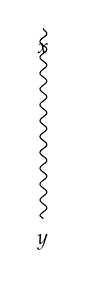
\begin{tikzpicture}[baseline={([yshift=1.4ex]current bounding box.center)}]
      \begin{feynman}[inline=(a)]
        \vertex (a);
        \vertex (b);
        \diagram {
          a -- [photon] b,
        };
        \vertex [below=0.2em of a] {\(_{x}\)};  
        \vertex [below=0.2em of b] {\(_{y}\)};  
      \end{feynman}
    \end{tikzpicture}\, .
\end{align}
The photon propagator is usually represented by a wavy line, as shown
in the second line above. 

\end{document}


\chapter{Divergences II --- the Vertex Function}
\label{cha:diverg-ii-vert}

% !TeX root = ./notes.tex
\documentclass[notes]{subfiles}

\setcounter{chapter}{6}



\begin{document}

\chapter{Divergences I --- the Scalar Propagator}
\label{cha:divergences-i-scalar}

\section{A first look at divergences}
\label{sec:a-first-look}

In this lecture we will aim to develop a self-consistent treatment of
divergences in QFT. This is a vast topic, which can hardly be
addressed exhaustively in the time that we have. Therefore we will
follow the following steps.
\begin{enumerate}
\item Compute the scalar two-point function beyond the first order in
  perturbation theory. As we try to perform this calculation we will
  encounter our first divergent integral.
\item Discuss the regularization of divergences; \ie a procedure that
  allows us to manipulate well-defined mathematical expressions, and
  to identify the structure of the divergences.
\item Discuss the renormalization of divergences; \ie the conditions
  that are necessary for a quantum field theory to produce finite,
  unambiguous predictions. 
\end{enumerate}

\subsection{Two-point function in perturbation theory}
\label{sec:scalar-two-point}

Working in perturbation theory, we compute the two-point function
\begin{equation}
  \label{eq:TwoPtMom}
  \tilde{G}^{(2)}\left(p,p'\right) =
  (2\pi)^D \delta\left(p+p'\right) \frac{1}{i} \tilde{\Delta}_F(p)\, ,
\end{equation}
as a Taylor expansion in powers of the coupling constant
\begin{equation}
  \label{eq:TwoPtMomPert}
  \tilde{G}^{(2)}\left(p,p'\right) = \sum_k g^k
  \tilde{G}^{(2,k)}\left(p,p'\right)\, .
\end{equation}
As discussed before, the delta function in Eq.~\ref{eq:TwoPtMom}
ensures momentum conservation. For all practical purposes, we should
remember that it is there, and work on the perturbative expansion of
the full propagator 
\begin{equation}
  \label{eq:PropMomPert}
  \tilde{\Delta}_F(p) = \sum_k g^k \tilde{\Delta}^{(k)}_F(p)\, .
\end{equation}
From our previous computations
\begin{align}
   \frac{1}{i} \tDelta_F^{(2)}(p)
  &= -\frac{1}{2} \SProp{p} \left(\int \frac{d^D\ell}{(2\pi)^D}\,
    \SProp{\ell} \SProp{(\ell-p)}\right) \times \nonumber \\
  &\quad \times \SProp{p}\, .,
\end{align}
and therefore the $O(g^2)$ contribution to the correlator can be
written as
\begin{equation}
  \label{eq:OneLoopPi}
  \frac{1}{i} \tDelta(p) \left(i\Pi(p^2)\right) \frac{1}{i}
  \tDelta(p)\, ,
\end{equation}
where
\begin{equation}
  \label{eq:PiFun}
  i\Pi(p^2) = \frac{g^2}{2} \int  \frac{d^D\ell}{(2\pi)^D}\,
  \SProp{\ell} \SProp{(\ell-p)}\, .
\end{equation}

\subsection{Evaluation of $\Pi(p^2)$}
\label{sec:evaluation-pi}

\paragraph{Feynman parameters}

The product of propagators in Eq.~(\ref{eq:PiFun}) can be rewritten
using Feynman parameters. The general formula
\begin{align}
  \frac{1}{A_1^{\alpha_1} \ldots A_n^{\alpha_n}}
  = & \frac{\Gamma(\alpha_1+\ldots +\alpha_n)}{\Gamma(\alpha_1)\ldots
      \Gamma(\alpha_n)}\, \int_0^1 dx_1\, x_1^{\alpha_1 -1} \ldots
      \int_0^1 dx_n\, x_n^{\alpha_n -1} \nonumber \\
    & \quad \times \delta\left(1-x_1-\ldots -x_n\right)\,
      \frac{1}{\left(x_1 A_1 + \ldots + x_n
      A_n\right)^{\alpha_1 + \ldots + \alpha_n}}\, , 
\end{align}
can be applied to the integrand above, yielding
\begin{align}
  \SProp{\ell} \SProp{(\ell-p)} = \int_0^1dx\,
  \frac{1}{\left(q^2-M^2 +i\epsilon\right)}\, ,
\end{align}
where $q=\ell-xp$, and $M^2(x,p)=m^2-x(1-x)p^2$. Hence, we have
\begin{equation}
  \label{eq:PiAfterFeynPar}
  i\Pi(p) = \frac{g^2}{2} \int_0^1dx\, \int \frac{d^Dq}{(2\pi)^D}\, 
  \frac{1}{\left(q^2-M^2 +i\epsilon\right)^2}\, .
\end{equation}

\paragraph{Wick rotation}

It is useful to introduce Euclidean momenta in order to perform the
integration. Because of the location of the poles, we can rotate the
integration contour clockwise by $\nicefrac{\pi}{2}$ to run along the purely
imaginary axis. Introducing
\begin{equation}
  \label{eq:EuclideanMom}
  q^0 = i q^0_E\, , \quad \mathbf{q} = \mathbf{q}_E\, ,
\end{equation}
we can rewrite
\begin{equation}
  \label{eq:PiEuclMom}
  \Pi(p^2) = \frac{g^2}{2} \int_0^1dx\, \int \frac{d^Dq_E}{(2\pi)^D}\, 
  \ESProp{q_E}{2}\, .
\end{equation}

\paragraph{A comment on divergences}

The integral in Eq.~(\ref{eq:PiEuclMom}) is clearly divergent for
$D\geq 4$. In particular, it is quadratically divergent in the UV for
the case $D=6$, which is the one we will be interested in. Before
developing more sophisticated tool, we can make a simple, but rather
deep, observation. If we take the derivative of $\Pi(p^2)$ with
respect to $p^2$:
\begin{equation}
  \label{eq:PiPrimeInt}
  \Pi'(p^2) = -g^2 \int_0^1dx\, x(x-1) \int \frac{d^Dq_E}{(2\pi)^D}\,
  \ESProp{q_E}{3}\, ,
\end{equation}
which is still divergent, but only for $D\geq 6$. Similarly
\begin{equation}
  \label{eq:PiDoublePrimeInt}
  \Pi''(p^2) = 3g^2 \int_0^1dx\, x^2(x-1)^2 \int \frac{d^Dq_E}{(2\pi)^D}\,
  \ESProp{q_E}{4}
\end{equation}
is divergent only for $D\geq 8$, and in particular is finite for
$D=6$. Therefore the function $\Pi(p^2)$ can be reconstructed by
integrating its second derivative twice,
\begin{equation}
  \label{eq:IntTwicePi}
  \Pi(p^2) = \Pi(\mu_1^2) + \Pi'(\mu_2^2) \left(p^2-\mu_1^2\right) +
  \int_{\mu_1^2}^{p^2} ds'\, \int_{\mu_2^2}^{s'} ds\, \Pi''(s)\, .  
\end{equation}
Eq.~(\ref{eq:IntTwicePi}) shows clearly that $\Pi(p^2)$ in $D=6$ is well
defined for all values of $p^2$ provided we fix the values of
$\Pi(\mu_1^2)$, and $\Pi'(\mu_2^2)$, \ie the values of the function
and its derivative at two \emph{arbitrary} values of the scale.

\section{Regularization}
\label{sec:regularization}

In order to make progress in our understanding of these divergences,
we need to first regulate the theory, \ie we need to choose a
prescription that makes the loop integrals mathematically well
defined. This is clearly a necessary condition in order to be able to
manipulate these expressions, and eventually define a predictive
theory that yields finite results for physical quantities.

There are several ways of regularizing the theory, here we list some
of the most common procedures, some of which we will explore in
tutorials.
\begin{enumerate}
\item Sharp cutoff in Euclidean momenta, $q_E^2\leq \Lambda^2$.
\item Pauli-Villars regulator. The propagators are modifed in order to
  have a less divergent behaviour at large values of the momenta:
  \begin{equation}
    \label{eq:PVReg}
    \SProp{p} \mapsto \SProp{p} - \frac{1}{p^2-M^2+i\epsilon}\, ,
  \end{equation}
  where $M$ is a mass scale that plays the role of the UV cutoff.
\item Schwinger-time regularization -- see PS7.
\item Work in generic dimension $D$, and define the divergent
  integrals by analytical continuation. 
\end{enumerate}

\subsection{Dimensional Regularization}
\label{sec:dimens-regul}

In dimensional regularization (DimReg), loop integrals are computed in
a generic dimension $D$, where the integration is actually
convergent, and then defined for arbitrary values of $D$ by analytical
continuation. Let us look at the integral that we encountered above
for the two-point function. After Wick rotation, we are interested in
\begin{equation}
  \label{eq:FirstExDimReg}
  I_D = \int \frac{d^Dq_E}{(2\pi)^D}\, \ESProp{q_E}{2}\, ,
\end{equation}
which is easily computed in spherical coordinates:
\begin{align}
  I_D &= \int \frac{d\Omega_D}{(2\pi)^D}\,
        \frac12 \int_0^\infty \dd{q_E^2}\, (q_E^2)^{\nicefrac{D}{2}-1} \ESProp{q_E}{2}
  \\
      &= \frac{1}{(2\pi)^{\nicefrac{D}{2}}} \frac{2\pi^{\nicefrac{D}{2}}}{\Gamma(\nicefrac{D}{2})}\,
        \frac12 \left(\frac{1}{M^2}\right)^{2-\nicefrac{D}{2}} \int_0^1 d\xi \,
        \xi^{1-\nicefrac{D}{2}} (1-\xi)^{\nicefrac{D}{2}-1} \\
  \label{eq:IDResult}
      &= \frac{1}{(4\pi)^{\nicefrac{D}{2}}} \frac{\Gamma(2-\nicefrac{D}{2})}{\Gamma(2)}
        \left(\frac{1}{M^2}\right)^{2-\nicefrac{D}{2}}\, .
\end{align}

\paragraph{Mathematical aside}

In deriving the above result we have made use of a number of useful
properties/tricks, which we summarise here.

\begin{enumerate}
\item The solid angle in $D$ dimension is
  \begin{equation}
    \label{eq:SoliAngleDDim}
    \Omega_D = \int \dd{\Omega_D} =
    \frac{2\pi^{\nicefrac{D}{2}}}{\Gamma(\nicefrac{D}{2})}\, .
  \end{equation}
\item We made a change of integration variable:
  \begin{equation}
    \label{eq:IntegVarChange}
    \xi = \frac{M^2}{q_E^2+M^2}\, .
  \end{equation}
\item The Euler gamma function is defined as
  \begin{equation}
    \label{eq:GammaFunDef}
    \Gamma(z) = \int_0^\infty dt\, t^{z-1} e^{-t}\, .
  \end{equation}
\item It can be readily shown that
  \begin{equation}
    \label{eq:GammRec}
    \Gamma(z+1) = z \Gamma(z)\, .
  \end{equation}
\item The beta function (Euler integral of the first kind) is defined
  as
  \begin{equation}
    \label{eq:BetaFunDef}
    B(\alpha,\beta) = \frac{\Gamma(\alpha)
      \Gamma(\beta)}{\Gamma(\alpha+\beta)} =
    \int_0^1 d\xi\, \xi^{\alpha-1} \left(1-\xi\right)^{\beta-1}\, .
  \end{equation}
\item For $n\geq 0$, and small $\epsilon$, we have
  \begin{align}
    \Gamma(n+1) &= n! \, , \\
    \Gamma\left(n+\frac12\right) &= \frac{(2n)!}{n!2^{(2n)}}
                                   \sqrt{\pi}\, , \\
    \Gamma(-n+\epsilon) &= \frac{(-)^n}{n!} \left[
                          \frac{1}{\epsilon} - \gamma + \sum_{k=1}^n
                          \frac{1}{k} + O(\epsilon)
                          \right]\, ,
  \end{align}
  where $\gamma=0.5772...$ is the Euler-Mascheroni constant. 
\end{enumerate}

\paragraph{Divergences of $I_D$}

Eq.~(\ref{eq:IDResult}) provides an expression for $I_D$ which can be
extended by analytical continuation to arbitrary values of $D$. It is
interesting to note that the divergences that we identified in $D=4$
and $D=6$ appear in the regularized version as poles of the gamma
function for negative integer values of its argument. 

\paragraph{General formula}

It is useful to generalise the result in Eq.~(\ref{eq:IDResult}):
\begin{equation}
  \boxed{
  \int \frac{d^Dq_E}{(2\pi)^D}\,
  \frac{\left(q_E^2\right)^a}{\left(q_E^2+M^2\right)^b}
  = \frac{\Gamma(b-a-\nicefrac{D}{2}) \Gamma(a+\nicefrac{D}{2})}{(4\pi)^{\nicefrac{D}{2}} \Gamma(b)
  \Gamma(\nicefrac{D}{2})} \left(M^2\right)^{-(b-a-\nicefrac{D}{2})}\, .}
\end{equation}
Manipulations similar to the ones above allow you to derive the
general formula. 

\subsection{Structure of divergences}
\label{sec:struct-diverg}

Let us now consider the case $D=6$, and work out in more detail the
structure of the divergences that appear in $\Pi(p^2)$. As discussed
above, for $D=6$ the integral $I_D$ is logarithmically divergent, and
therefore it is convergent as soon as $D<6$. We will therefore use
dimensional regularization, and define the integral in
$D=6-2\epsilon$.

Before we start manipulating the integral, we need to do some
dimensional analysis first. For $D=6$, the scalar field has mass
dimensions
\[
  \left[\phi\right] = \frac{D-2}{2}= 2\, ,
\]
and therefore the coupling constant $g$ is dimensionless. This is a
useful property that we want to preserve; as we continue our
expressions to $D=6-2\epsilon$ we replace $g$ in the action by
$g\tilde{\mu}^\epsilon$, where $\tilde{\mu}$ is an arbitrary scale,
and $g$ remains a dimensionless coupling. This seemingly harmful
rescaling has deep consequences: the regularization procedure -- in
this case changing the number of space-time dimensions -- has
automatically introduced a new scale in the problem.

With these choices for the regulator, we find
\begin{align}
  \Pi(p^2) = \frac12 \alpha \Gamma(\epsilon-1) \int_0^1dx\,
  M^2(x,p^2)
  \left(\frac{4\pi\tilde{\mu}^2}{M^2(x,p^2)}\right)^\epsilon\, .
\end{align}

\paragraph{$\epsilon$ dependence}

We can now compute explicitly the dependence on $\epsilon$:
\begin{align}
  \Gamma(\epsilon-1) &= -\left[
                       \frac{1}{\epsilon} - \gamma + 1 +O(\epsilon)
                       \right] \, , \\
  \left(\frac{4\pi\tilde{\mu}^2}{M^2(x,p^2)}\right)^\epsilon
                     &= 1 + \epsilon \log
                       \left(\frac{4\pi\tilde{\mu}^2}{M^2(x,p^2)}\right)
                       + O(\epsilon^2)\, ,
\end{align}
and hence
\begin{align}
  \Gamma(\epsilon-1)
  \left(\frac{4\pi\tilde{\mu}^2}{M^2(x,p^2)}\right)^\epsilon
  &= - \left[
    \frac{1}{\epsilon} - \gamma +1 + \log
    \left(\frac{4\pi\tilde{\mu}^2}{M^2(x,p^2)}\right) 
    + O(\epsilon)
    \right]\, .
\end{align}
Collecting all contributions yields
\begin{align}
  \Pi(p^2) &= -\frac{\alpha}{2} \int_0^1 dx\,
             M^2(x,p^2) \left[
             \frac{1}{\epsilon} +1 + \log
             \left(\frac{4\pi\tilde{\mu}^2}{e^\gamma M^2(x,p^2)}\right) 
    + O(\epsilon)
             \right] \\
  \label{eq:ExplicitDivs}
           &= \frac{\alpha}{2} \left[
             \left(\frac{1}{\epsilon}+1\right) \left(\frac{1}{6}
             p^2-m^2\right)
             - \int_0^1dx\, M^2(x,p^2) \log\left(\frac{\mu^2}{M^2}\right)
             \right]
             +O(\epsilon) \, ,
\end{align}
where
\begin{equation}
  \label{eq:DefAlpha}
  \alpha = \frac{g^2}{(4\pi)^3}\, , \quad \mu^2 =
  \frac{4\pi}{e^\gamma} \tilde{\mu}^2\, .
\end{equation}
Eq.~(\ref{eq:ExplicitDivs}) shows explicitly the structure of the
divergences in the loop integral. They are given by the two terms
proportional to $1/\epsilon$, and are proportional to $p^2$ and
$m^2$. Understanding the structure of the divergent terms is the first
step to be able to understand how to treat them. For the time being,
we note that the divergent terms look like the contribution to the
propagator that one would obtain from interaction vertices in the
lagrangian that contain only two fields, \ie vertices like
$\partial_\mu \phi \partial^\mu\phi$ and $\phi^2$. These vertices are
usually called \emph{counter terms}.

\paragraph{A geometric series}

Having evaluated $\Pi(p^2)$, we can easily re-sum an entire class of
contributions:
\begin{align}
  \label{eq:PiGeometricSeries}
  \frac{1}{i} \tDelta_F(p^2)
  =&\, 
     \begin{tikzpicture}[baseline=\plusheight]
       \begin{feynman}
         \vertex (a);
         \vertex [right= 1.0cm of a] (b);
         \diagram [horizontal=a to b, layered layout] {
           (a) --(b)
         };
       \end{feynman}
     \end{tikzpicture}
     +
     \begin{tikzpicture}[baseline=\plusheight]
       \begin{feynman}
         \vertex (a);
         \vertex [left=0.5cm of a] (i1);
         \vertex [right= 1.0cm of a] (b);
         \vertex [right=0.5cm of b] (f1);
         \diagram [horizontal=a to b, layered layout] {
           (i1) -- (a)
           -- [half left] (b) 
           -- [half left] (a) ,
           (f1) --(b)
         };
       \end{feynman}
     \end{tikzpicture}
     +
     \begin{tikzpicture}[baseline=\plusheight]
       \begin{feynman}
         \vertex (a);
         \vertex [left=0.5cm of a] (i1);
         \vertex [right= 1.0cm of a] (b);
         \vertex [right=0.5cm of b] (f1);
         \vertex [right= 1.0cm of f1] (b1);
         \vertex [right=0.5cm of b1] (f2);
         \diagram [horizontal=a to b, layered layout] {
           (i1) -- (a)
           -- [half left] (b) 
           -- [half left] (a) ,
           (b) --(f1)
           -- [half left] (b1)
           -- [half left] (f1),
           (b1) -- (f2);
         };
       \end{feynman}
     \end{tikzpicture}
     + \ldots \\
  =& \frac{1}{i} \tDelta(p^2) +
     \frac{1}{i} \tDelta(p^2) \left[\left(i \Pi(p^2)\right)
     \left(\frac{1}{i} \tDelta(p^2) \right) \right] + \nonumber \\
  & \quad\quad + 
     \frac{1}{i} \tDelta(p^2) \left[\left(i \Pi(p^2)\right)
     \left(\frac{1}{i} \tDelta(p^2) \right) \right]^2 +
    \ldots \\
  =& \frac{1}{i} \tDelta(p^2) \; \sum_{k=0}^\infty \left[\Pi(p^2)
     \tDelta(p^2)\right]^k \\ 
  =&  \frac{1}{i} \tDelta(p^2)\; \frac{1}{1-\Pi(p^2) \tDelta(p^2)}\, .
\end{align}
Hence the net result of the sum yields
\begin{equation}
  \label{eq:FullPropOneLoop}
  \tDelta_F(p^2) = \frac{1}{p^2-m^2-\Pi(p^2) + i\epsilon}\, ,
\end{equation}
where we have reintroduced the $i\epsilon $ term in the denominator
(not to be confused with the parameter $\epsilon $ of DimReg).

\paragraph{Comparison with K-L}

According to the Källén-Lehmann representation of the propagator, we
expect to find a pole for $p^2=\mphys^2$, with the corresponding
residue being equal to one. Two observations are in order.
\begin{enumerate}
\item 
  In order to have such a pole we need
  \begin{equation}
    \label{eq:MphysPole}
    \mphys^2 - m^2 - \Pi(\mphys^2) = 0
  \end{equation}
  to hold, which clearly shows that $\mphys^2\neq m^2$.
\item
  Similarly we can
  compute the residue of the propagator at $p^2=\mphys^2$ by expanding
  the denominator in $p^2$ around $\mphys^2$,
  \begin{equation}
    \label{eq:ResDenExp}
    p^2-m^2-\Pi(p^2) =
    \left(p^2 - \mphys^2\right) \left[1 - \Pi'(\mphys^2)\right] +
    O\left(\left(p^2 - \mphys^2\right)^2\right)\, ,
  \end{equation}
  which in turn yields
  \begin{align}
    \mathrm{Res}_{\mphys^2} \tDelta(p^2)
    &= \lim_{p^2\to\mphys^2} \left(p^2 - \mphys^2\right) \tDelta(p^2) \\
    &= \frac{1}{1 - \Pi'(\mphys^2)}\, .
  \end{align}
  The latter equation shows that the field $\phi$ that appears in the
  Lagrangian does not have the normalization required to agree with the
  K-L representation.
\end{enumerate}
These two observations suggest a general line of thinking: the fields
and couplings that appear in the Lagrangian, the so-called \emph{bare
  fields} and \emph{bare coupings} are not physical. The physical
variables need to be defined according to some well-specified
prescription. The process of specifying these quantities is known as
\emph{renormalization} of the theory.

\section{Renormalization}
\label{sec:renormalization}

\subsection{Renormalized perturbation theory}
\label{sec:renorm-pert-theory}

\paragraph{Renormalization of the field}

As suggested by the comparison with K-L, we define a {\em
  renormalized field}
\begin{equation}
  \label{eq:RenormField}
  \phi(x) = Z^{\nicefrac{1}{2}} \phi_R(x)\, ,
\end{equation}
where $Z$ is the renormalization constant of the field.  In terms of
the new field the Lagrangian is
\begin{align}
  \mathcal{L}= \frac12 \partial_\mu \phi_R \partial^\mu \phi_R -
  \frac12 m^2 Z \phi_R^2 + \frac{g}{3!} Z^{\nicefrac{3}{2}} \phi_R^3 +
  \frac12 \delta_Z \partial_\mu \phi_R \partial^\mu \phi_R\, ,
\end{align}
where we have introduced $\delta_Z=Z-1$.

\paragraph{Renormalization of mass and coupling}

We can also introduce a renormalized mass and a renormalized coupling
\begin{equation}
  \label{eq:RenormMass}
  m^2 Z = Z_m m_R^2\, ,\quad g Z^{\nicefrac{3}{2}}= Z_g g_R
\end{equation}
where we have introduced two new renormalization constants $Z_m$ and
$Z_g$.

\paragraph{Renormalized perturbation theory}

We can rewrite the Lagrangian one more time as
\begin{align}
  \mathcal{L}= \frac12 \partial_\mu \phi_R \partial^\mu \phi_R -
  \frac12 m_R^2 \phi_R^2 + \frac{Z_g g_R}{3!} \phi_R^3 +
  \frac12 \delta_Z \partial_\mu \phi_R \partial^\mu \phi_R
  - \frac12 \delta_m \phi_R^2
  \, ,
\end{align}
where $\delta_m=Z_m-1$. The expression above for the Lagrangian looks
identical to the bare one, except that fields and couplings are now
renormalized, and there two counter terms proportional to $\delta_Z$
and $\delta_m$ respectively. We can therefore define the path integral
in terms of renormalized quantities; this will lead to 
\emph{renormalized perturbation theory}. 

We can now compute $\Pi(p^2)$ in renormalized perturbation theory, the
result is identical to the one obtained before, plus the contribution
of the counter terms:
\begin{equation}
  \label{eq:PiRenormPertTh}
  \Pi(p^2)=\frac{\alpha}{2}\left[
    \left(\frac{1}{\epsilon}+1\right)
    \left(\frac{1}{6}p^2-m_R^2\right) +
    \int_0^1dx\, M^2\log\left(\frac{M^2}{\mu^2}\right)
  \right] + \delta_Z p^2 - \delta_m m_R^2 + O(\alpha^2)\, .
\end{equation}
Is it useful to rewrite the equation above as:
\begin{align}
  \Pi(p^2)
  =& \frac{\alpha}{2}\int_0^1dx\,
     M^2\log\left(\frac{M^2}{m_R^2}\right) +
     \left[
     \frac{\alpha}{6} \left(\frac{1}{2\epsilon} + \log(\mu/m_R) +
     \frac12 \right) + \delta_Z
     \right] p^2 - \nonumber \\
   & - \left[
     \alpha\left(\frac{1}{2\epsilon} + \log(\mu/m_R) +
     \frac12 \right) + \delta_m
     \right] m_R^2 + O\left(\alpha^2\right)\, .
\end{align}
Note that at this stage we have not yet defined the renormalization
constants, and therefore $\delta_Z$ and $\delta_m$ are free parameters
that need to be fixed.  Note also that by choosing
\begin{align}
  \delta_z =& -\frac{\alpha}{6} \left(\frac{1}{2\epsilon} + \log(\mu/m_R) +
              \frac12 + \kappa_Z \right) + O\left(\alpha^2\right)\, , \\
  \delta_m =& -\alpha\left(\frac{1}{2\epsilon} + \log(\mu/m_R) +
     \frac12 + \kappa_m\right) + O\left(\alpha^2\right)\, , 
\end{align}
where $\kappa_Z$ and $\kappa_m$ are finite constants, we obtain a
value for $\Pi(p^2)$ which is finite when $\epsilon\to 0$, and
independent of the arbitrary scale $\mu$.

\paragraph{Renormalization conditions}

In order to fully determine the renormalization constants, we need to
specify a so-called \emph{renormalization scheme}. The renormalization
scheme is defined by imposing a number of conditions that are
sufficient to determine all the renormalization constants. Clearly these
conditions are necessary in order to have a predictive framework.

\subsection{Renormalization scheme}
\label{sec:renorm-scheme}

\end{document}


\chapter{Renormalization}
\label{cha:renormalization}
% \input{Sections/Renorm.tex}


\chapter{Renormalization Group}
\label{cha:renorm-group}

\chapter{Scales - Decoupling}
\label{cha:scales-decoupling}

\printindex
\end{document}

%%% Local Variables:
%%% mode: latex
%%% TeX-master: t
%%% End:
